\label{5_resultados}

\section{Parâmetros analisados}

Como um AG trabalha com tentativa-e-erro, não é possível prever quando se atingirá uma solução. Para se analisar a evolução dos indivíduos ao longo das gerações, este trabalho focou em analisar os seguintes parâmetros:

\begin{itemize}
	\item Valor mínimo de fitness em um indivíduo;
	\item Valor máximo de fitness em um indivíduo;
	\item Valor médio de fitness entre todos os indivíduos;
	\item Desvio padrão dos valores de fitness.
\end{itemize}

O desvio padrão utilizado aqui foi o amostral, dado por:

\begin{equation}
	\sigma = \sqrt{\frac{1}{N-1} \sum_{i=1}^N (x_i - \overline{x})^2}
\end{equation}

Este trabalho analisou o comportamento de tais valores em gráficos, os quais foram criados com base em uma única simulação do AG para cada conjunto (problema + parâmetros de entrada). Como não é possível prever valores, analisar o comportamento de tais curvas se mostrou mais valioso.

Se não for mencionado, utilizou-se 0.9 para $p_c$ e 0.01 para $p_m$. Todas as execuções utilizaram 100 indivíduos, 200 gerações e elitismo do melhor indivíduo. Se um problema convergiu toda sua população para a solução ótima antes de 200 gerações, os gráficos foram reduzidos para melhor visualização.

As simulações feitas com uso do AGA foram comparadas com as simulações do AG com parâmetros estáticos. Além disso, foi avaliado o comportamento adaptativo de $p_m$ ao longo das gerações.

\section{OneMax Booleano}

\subsection{Caso Estático}

Este problema foi considerado simples de ser resolvido por um AG, uma vez que poucas mutações em um gene já permitem que ele ficasse igual a 1. A figura \ref{fig:onemax_boolean} demonstra exatamente isso, com convergência completa dos indivíduos para a solução ótima após 93 gerações, sendo que a própria solução ótima foi encontrada com a melhor solução aparecendo após 78 gerações.

\begin{figure}[ht!]
    \centering 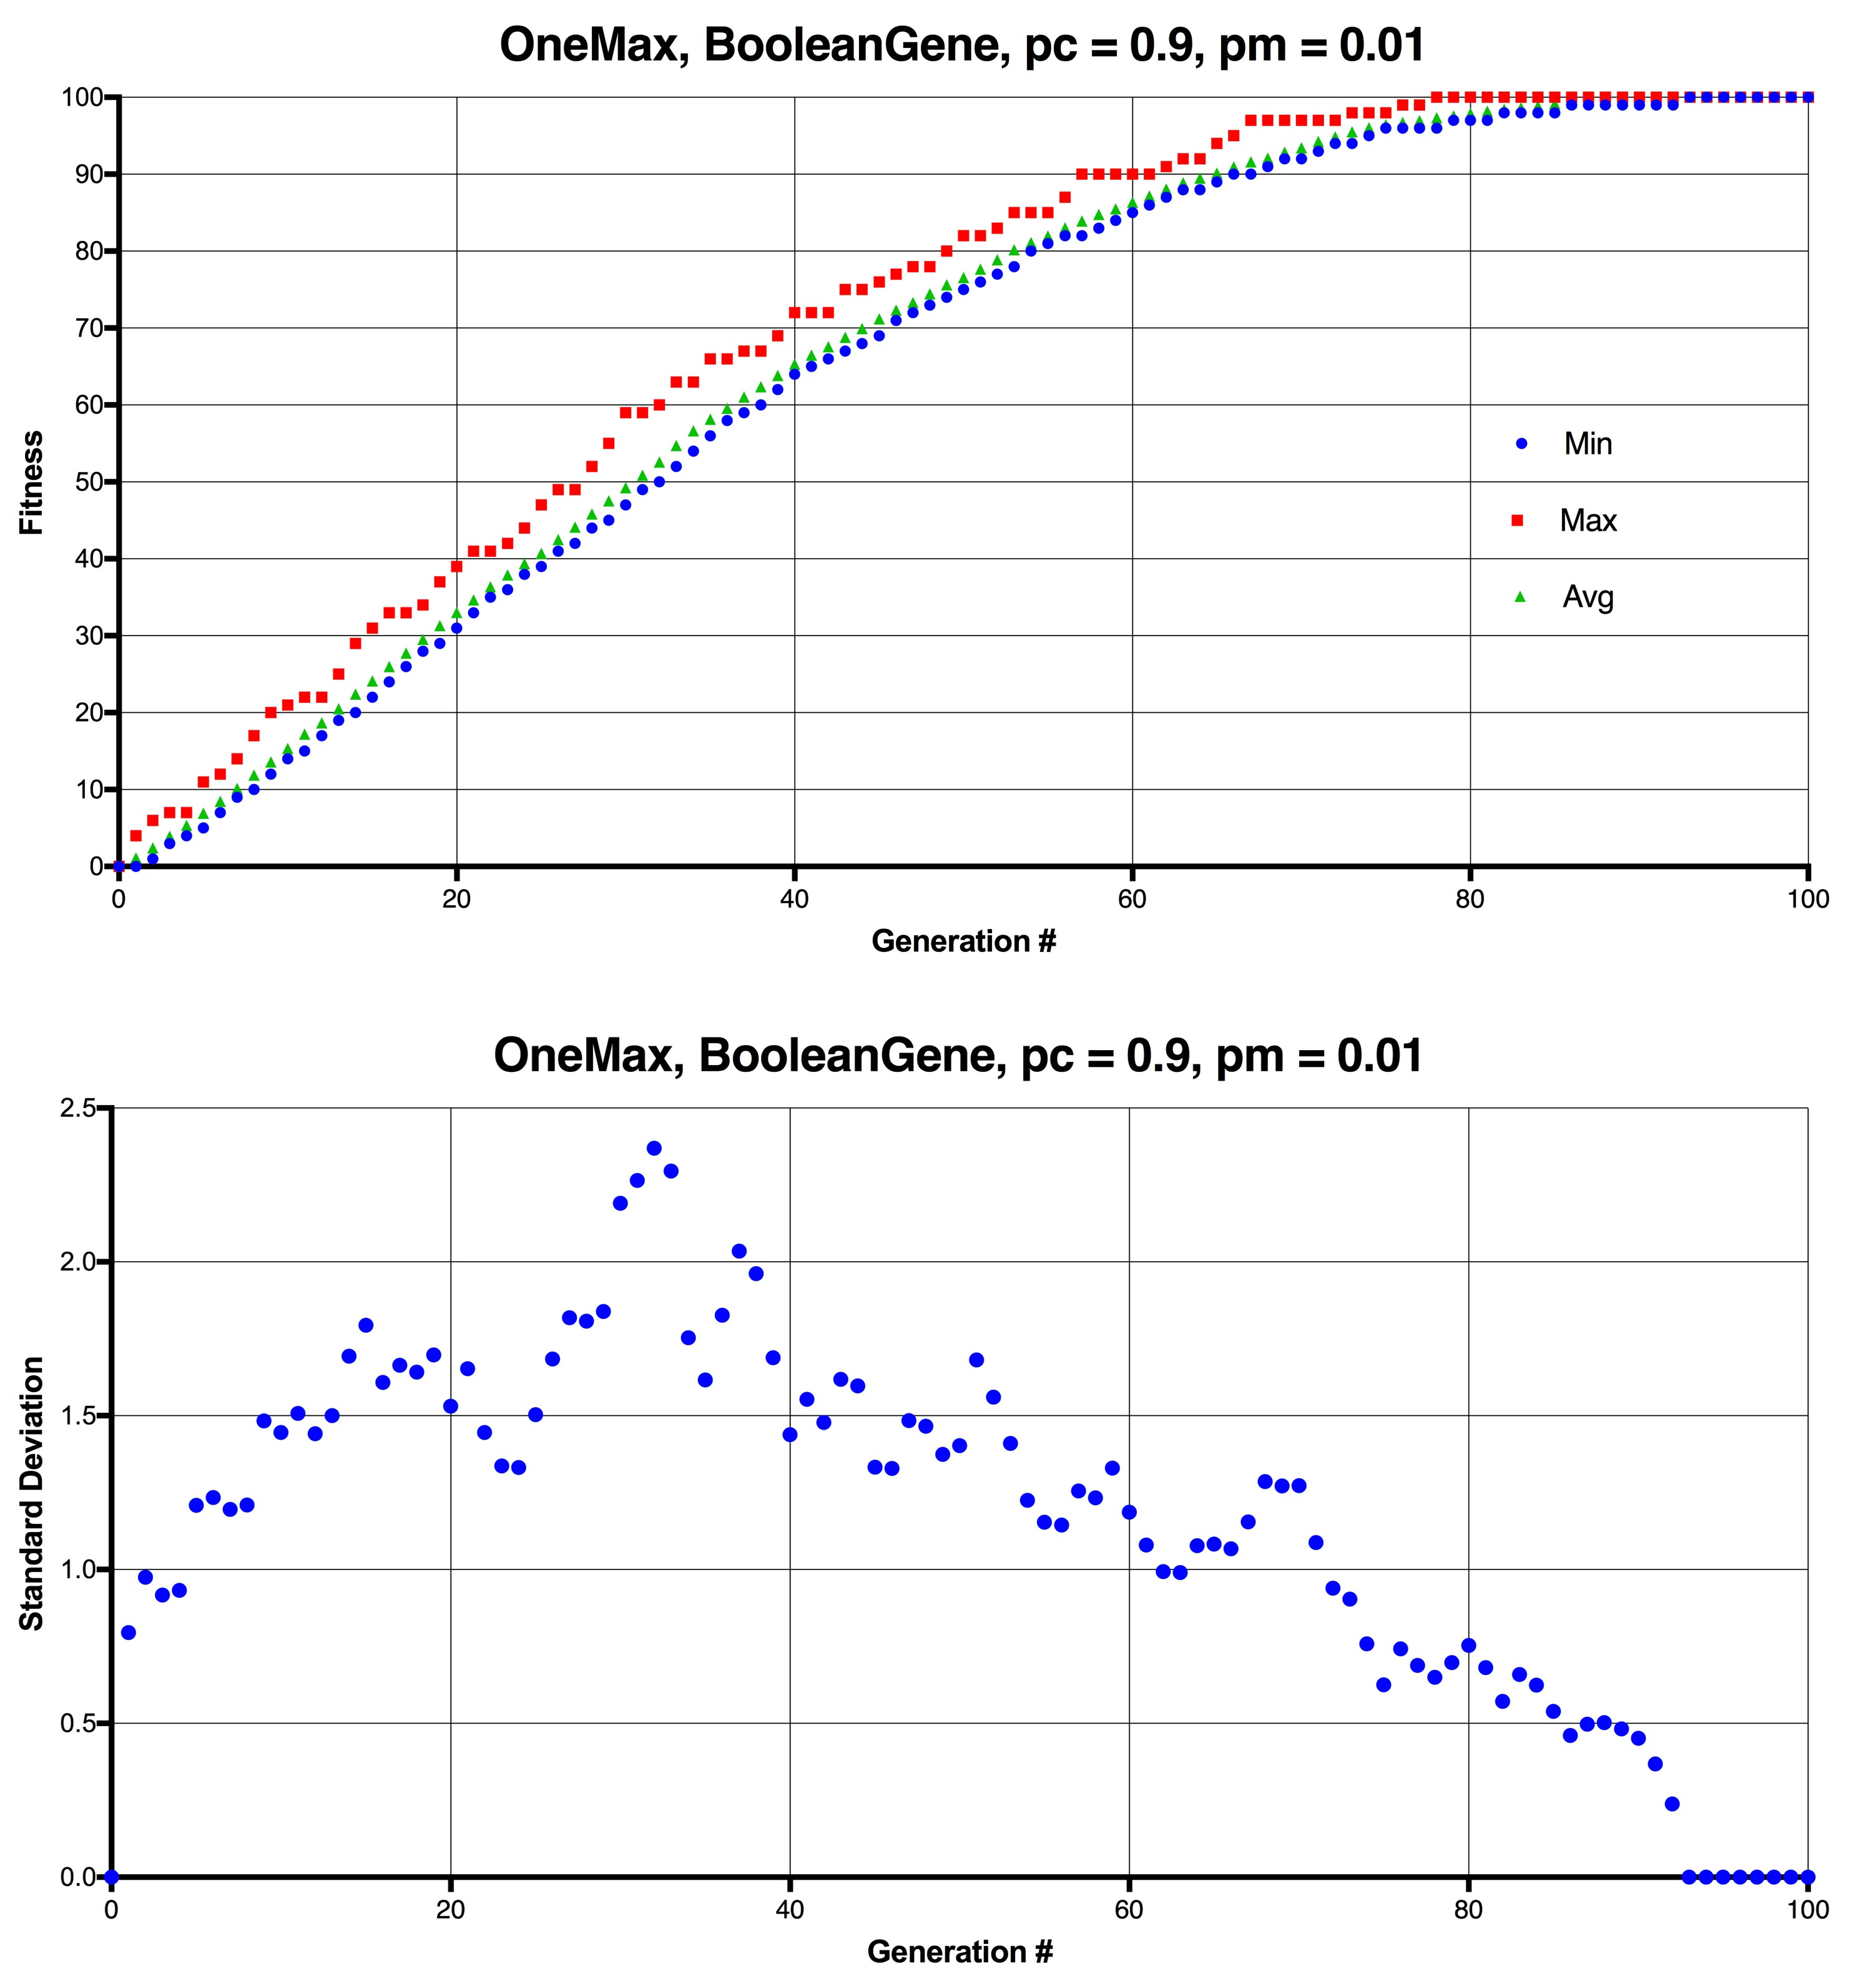
\includegraphics[width=1.0\textwidth]{onemax_boolean.jpg}
    \caption{Evolução do fitness para o problema do OneMax Booleano mostrando mínimo, máximo, valor médio e desvio padrão ($p_c=0.9$, $p_m=0.01$). Foram necessárias 78 gerações para que a solução ótima aparecesse, e 93 gerações para que a população inteira convergisse para ela.}
    \label{fig:onemax_boolean}
\end{figure}

O comportamento estático para os valores padronizados de $p_c$ e $p_m$ mostrou um crescimento aproximadamente linear dos valores de fitness de toda a população. Isso nos diz que os parâmetros presentes estão em equilíbrio, e a mutação presente é suficiente para uma boa convergência.

\subsection{Caso Adaptativo}

Com o AGA ativado, atingir a solução ótima demorou um pouco mais. Como mostrado na figura \ref{fig:onemax_boolean_adaptive}, foram necessárias 140 gerações para que o melhor indivíduo atingisse a solução ótima, enquanto a média da população nunca conseguisse convergir. O desvio padrão nunca passou de 2.0 (de um máximo de 100), o que nos diz que a população não se dispersou completamente pelo efeito adaptativo.

\begin{figure}[ht!]
    \centering 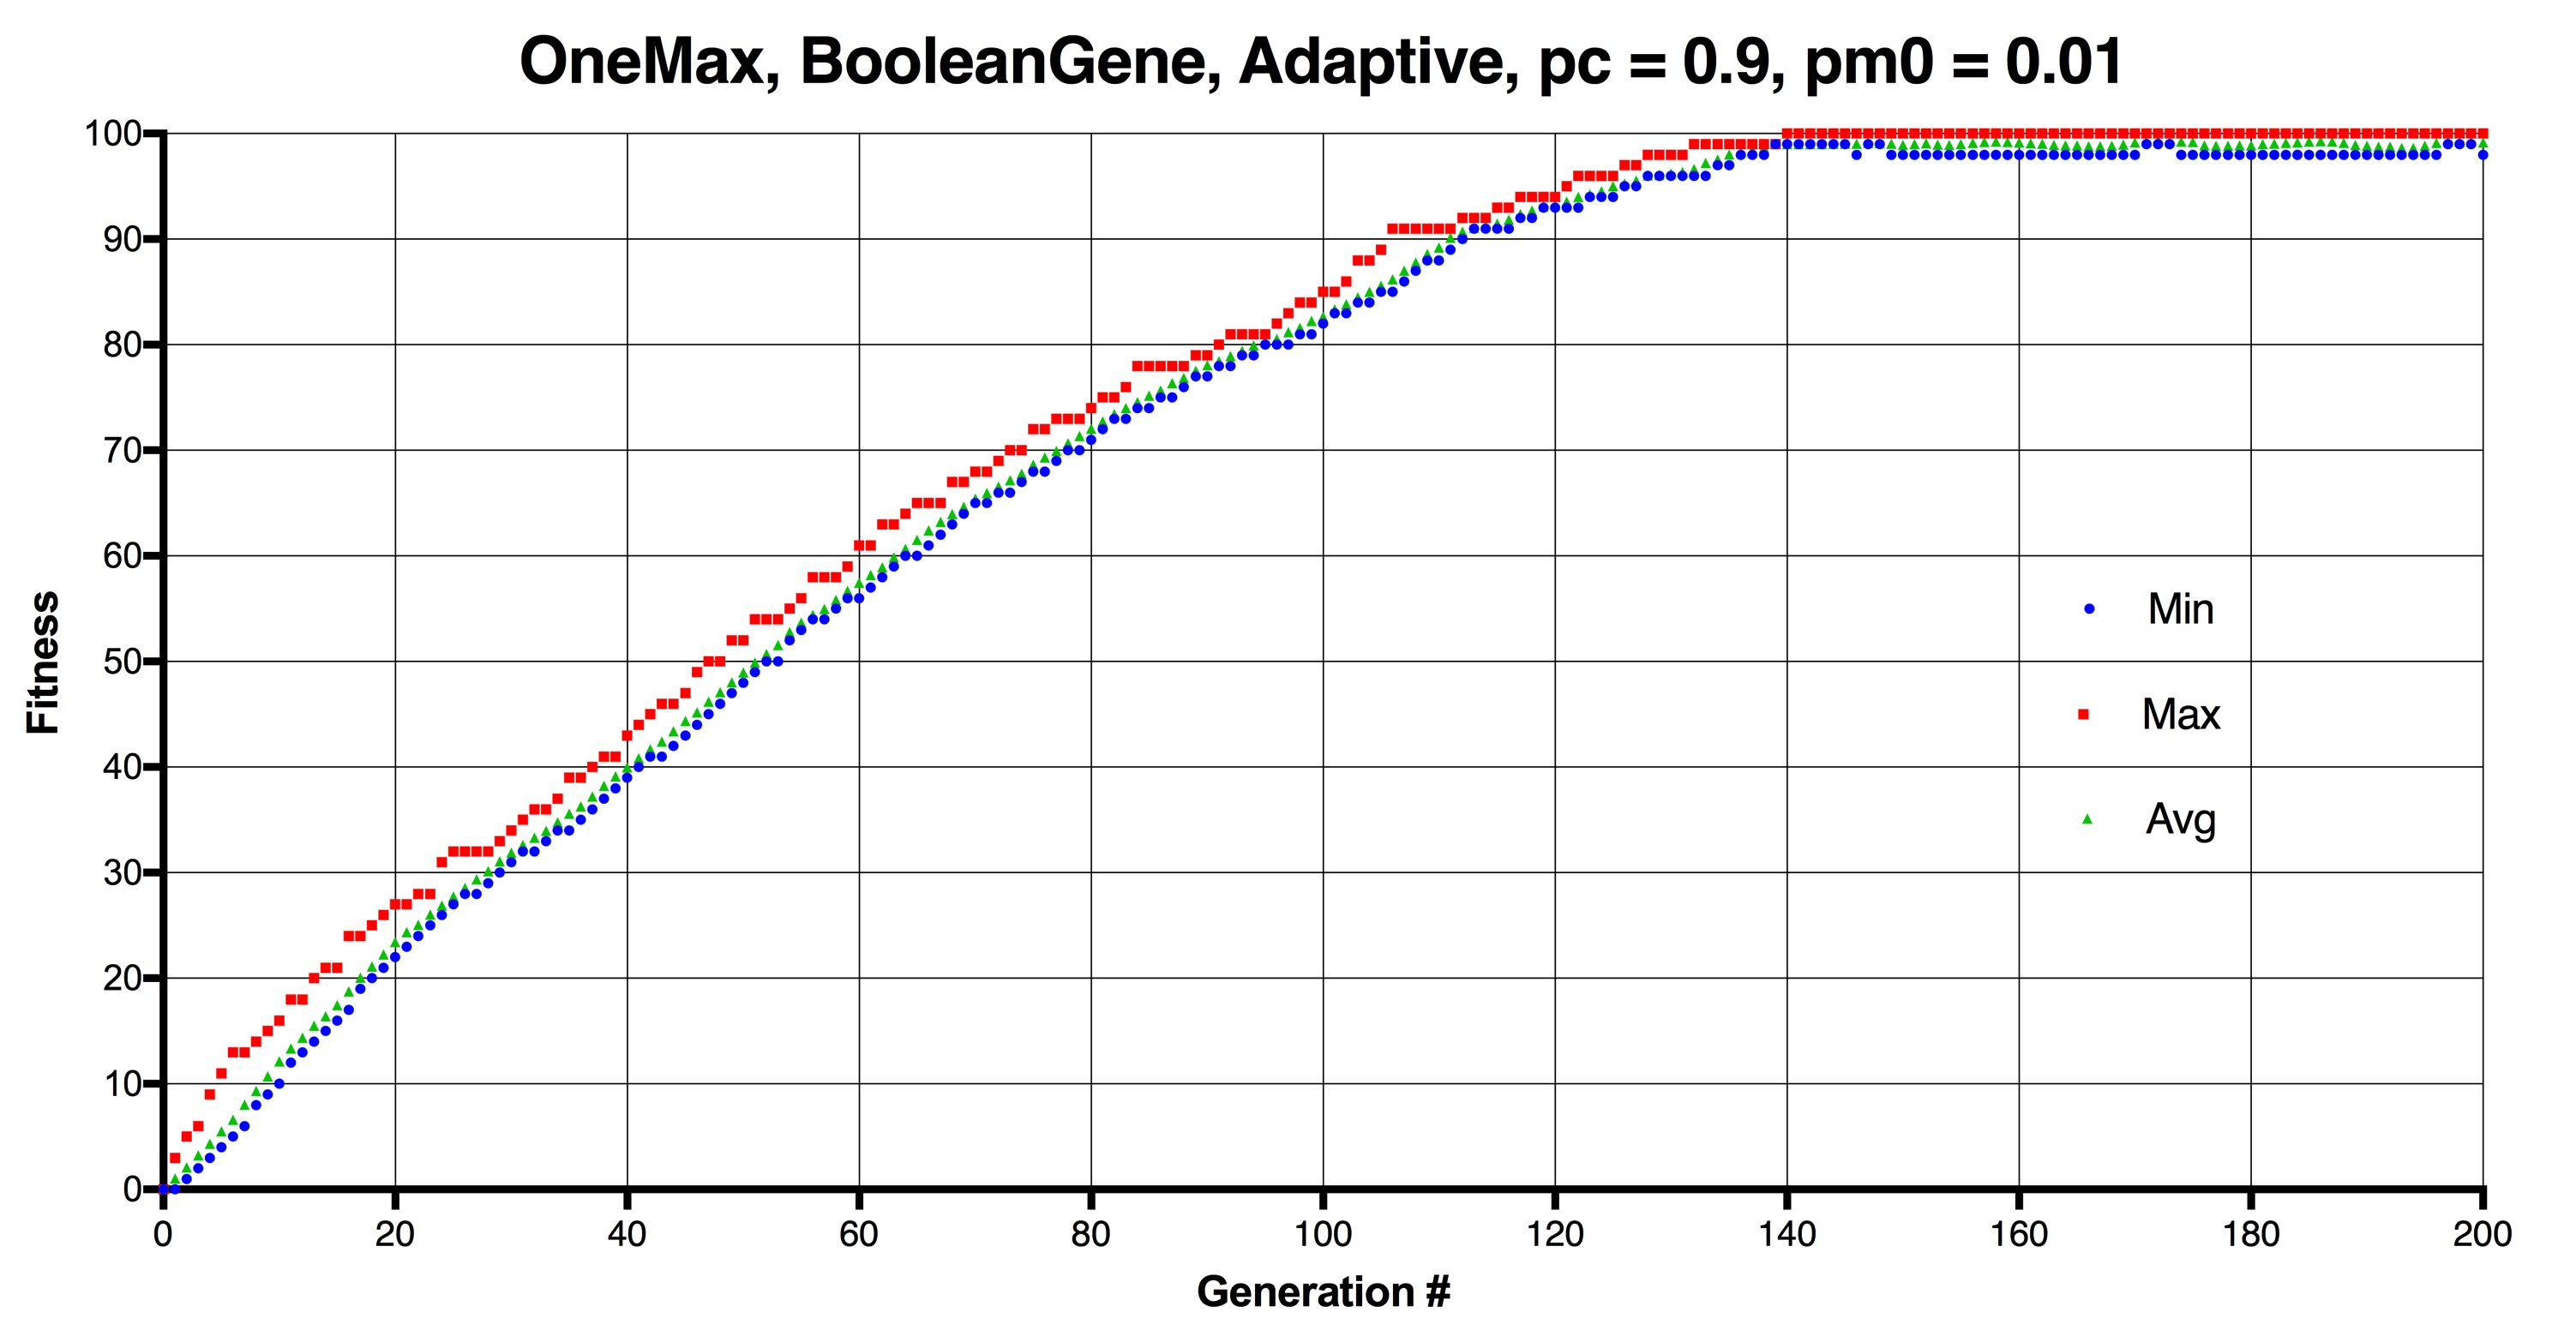
\includegraphics[width=1.0\textwidth]{onemax_boolean_adaptive.jpg}
    \caption{Evolução do fitness para o problema do OneMax Booleano Adaptativo mostrando mínimo, máximo, valor médio e desvio padrão ($p_c=0.9$, ${p_m}_0=0.01$). Foram necessárias 140 gerações para que um indivíduo encontrasse a solução ótima.}
    \label{fig:onemax_boolean_adaptive}
\end{figure}

O funcionamento do AGA com relação à evolução de $p_m$ pode ser visto com clareza na figura \ref{fig:onemax_boolean_adaptive_pm}. As primeiras gerações, por estarem ainda dispersas, fizeram com que $p_m$ diminuísse, o que fez com que a população descobrisse melhores soluções de modo mais lento (com isso, as 140 gerações).

\begin{figure}[ht!]
    \centering 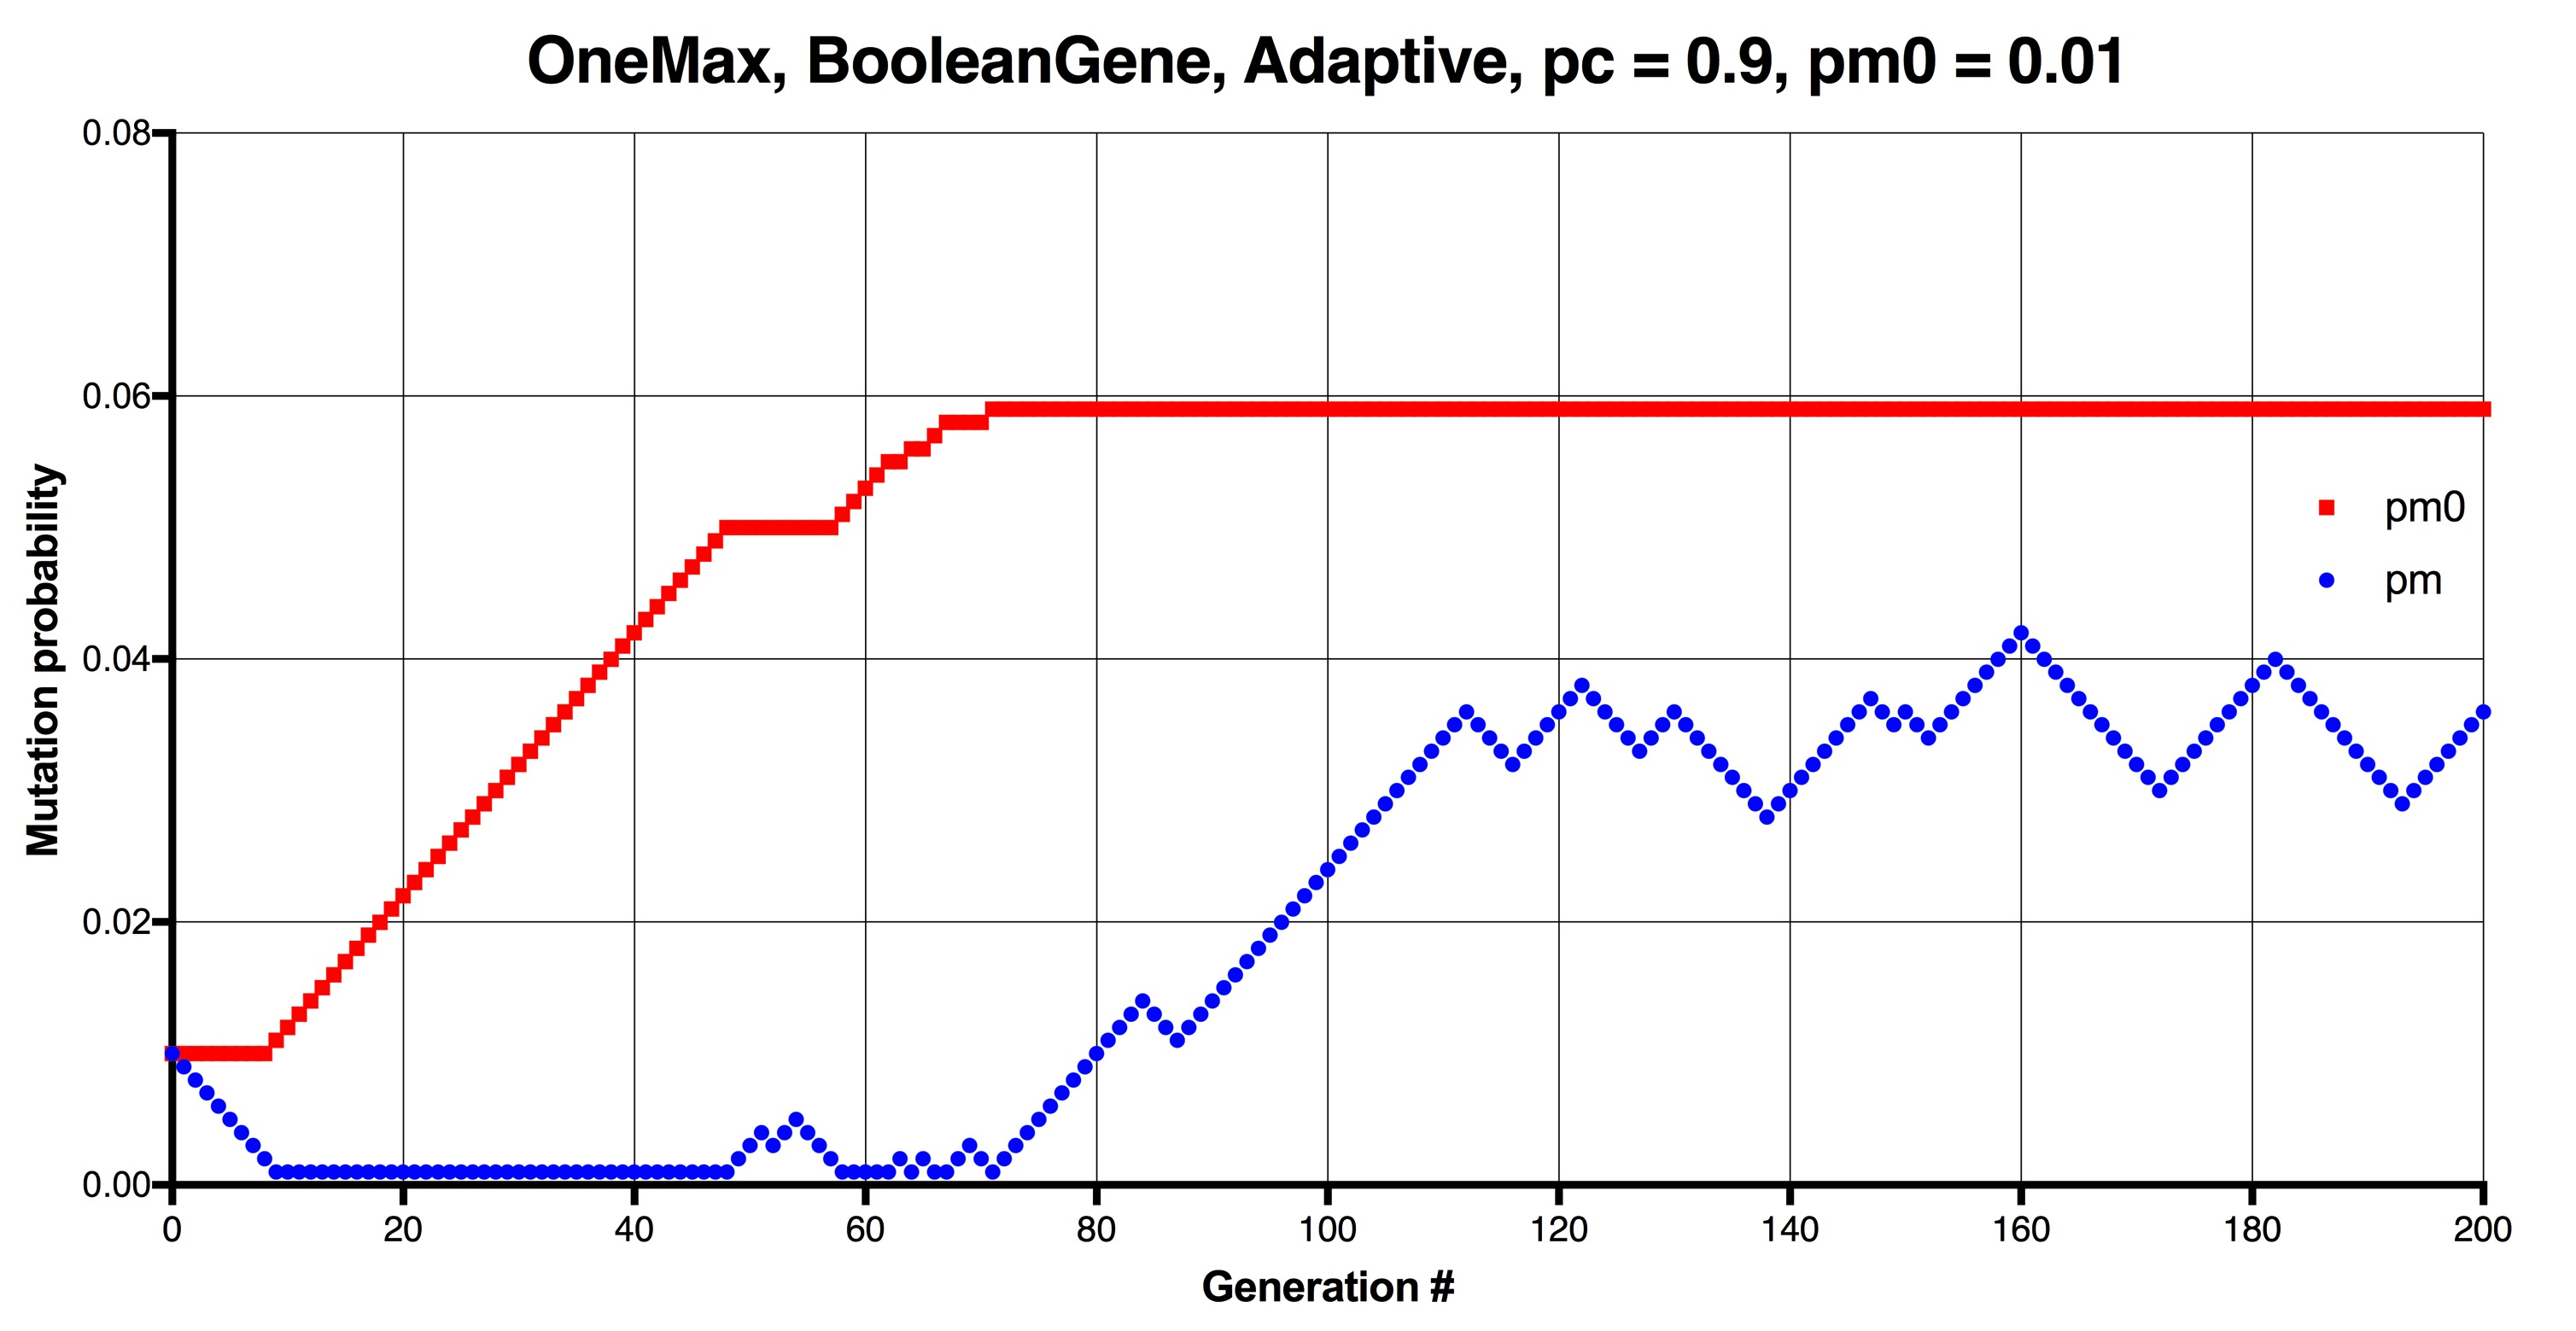
\includegraphics[width=1.0\textwidth]{onemax_boolean_adaptive_pm.jpg}
    \caption{Evolução da probabilidade de mutação $p_m$ ao longo das gerações, juntamente com o desvio do melhor valor de fitness com relação à média ($p_c=0.9$, ${p_m}_0=0.01$).}
    \label{fig:onemax_boolean_adaptive_pm}
\end{figure}

No entanto, sob baixa mutação, a população eventualmente se estabilizou (eventualmente chegando a desvio zero em 139 gerações), e $p_m$ começou a aumentar. Por conta de o AGA manter o desvio sempre em alta, mesmo depois de o melhor indivíduo encontrar a solução ótima, $p_m$ cresceu para um patamar maior que o original (em torno de 0.015), impedindo que a população obtivesse desvio zero.

Foi possível ver nesta simulação o comportamento mais básico deste AGA: o impedimento de uma convergência completa da população para uma mesma solução (mesmo que tal solução seja a ótima). Mesmo com este impedimento, ainda foi possível que o melhor indivíduo a encontrasse num tempo razoável.

Os dados de interesse vindos destas simulações podem ser encontrados na tabela \ref{tab:onemax_boolean}.

\begin{table}
\caption{Dados coletados do problema OneMax Booleano ($p_m = 0.01$).}
\label{tab:onemax_boolean}

\center
\begin{tabular}{|c|cc|}
	\hline
	Algoritmo analisado (AG = caso estático)				& AG		& AGA		\\
	\hline
	Solução ótima encontrada?								& Sim		& Sim		\\
	Gerações p/solução ótima								& $78$		& $140$		\\
	Convergência da população p/solução ótima (gerações)	& $93$		& $--$		\\
	Fitness médio após 100 gerações							& $100$		& $82.67$	\\
	Fitness médio após 200 gerações 						& $100$		& $99.17$	\\
	Valor final de $p_m$									& $0.01$ 	& $0.019$	\\
	Valor mínimo de $p_m$									& $0.01$	& $0.001$	\\
	Valor máximo de $p_m$									& $0.01$	& $0.021$	\\
	Valor médio de $p_m$									& $0.01$	& $0.00594$	\\
	Valor médio de $p_m$ (últimas 100 gerações)				& $0.01$	& $0.0105$	\\
	\hline
\end{tabular}
\end{table}

\section{OneMax Real}

Para o OneMax Real, é impossível chegar ao valor máximo de fitness (100.0), uma vez que a mutação para um número aleatório trabalha no intervalo [0, 1). Por conta disso, as análises feitas aqui focaram no comportamento da curva e na diferença de comportamento frente aos resultados do OneMax Booleano.

\subsection{Caso Estático}

Foi possível ver, na figura \ref{fig:onemax_real}, que a população, mesmo não sendo capaz de atingir o fitness máximo, conseguiu se homogeneizar e continuar crescendo de modo estável ao longo das gerações, o que foi demonstrado também pela queda do desvio padrão. Isso nos mostra que as populações de um problema OneMax evoluem melhor quando são mais homogêneas.

\begin{figure}[ht!]
    \centering 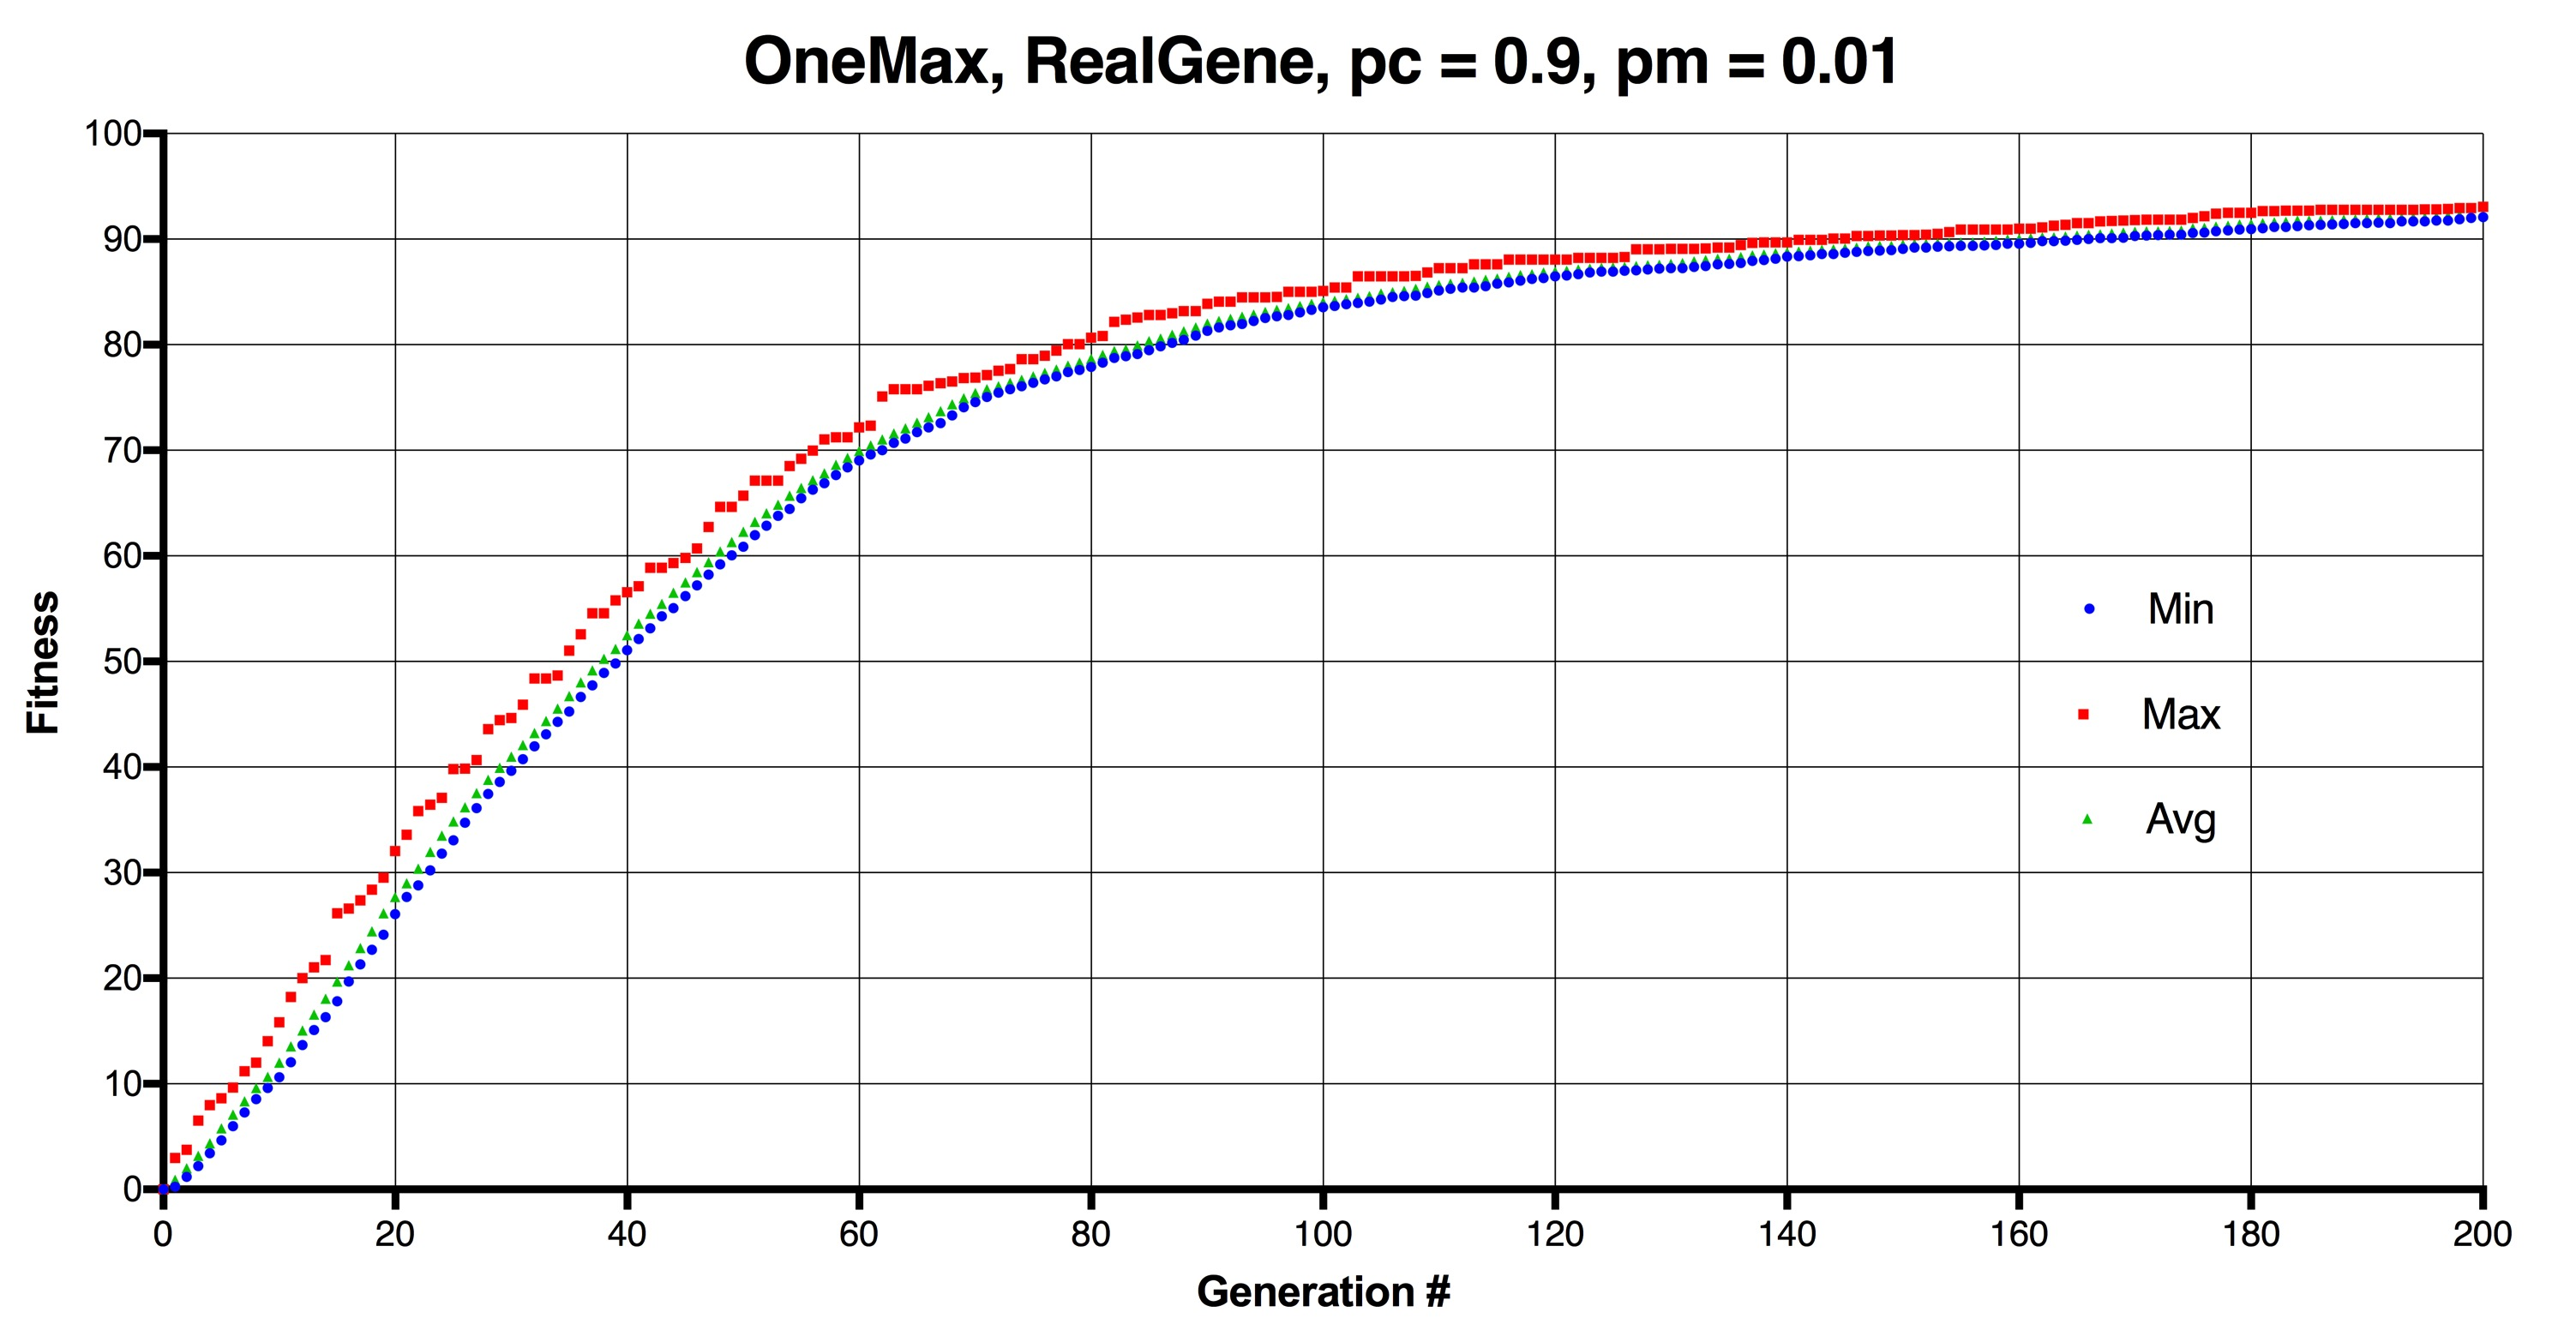
\includegraphics[width=1.0\textwidth]{onemax_real.jpg}
    \caption{Evolução do fitness para o problema do OneMax Real mostrando mínimo, máximo, valor médio  e desvio padrão ($p_c=0.9$, $p_m=0.01$).}
    \label{fig:onemax_real}
\end{figure}

Os pontos de qualquer uma das medições (média, mínimo e máximo) parecem formar uma curva. Descobri-la fugiu do escopo deste trabalho, mas tal formato pode estar associado à probabilidade de se aumentar a expressividade de um gene. Na execução deste AG, cada gene é levado para mutação com probabilidade $p_m$. Se um gene tiver uma expressividade $0 < x < 1$, a mutação (assumida uniforme) possui uma probabilidade $(1-x)$ de aumentá-la. Logo, a expressividade aumentará em uma dada geração com probabilidade:

\begin{equation}
	p_m(1-x)
\end{equation}

\subsection{Caso Adaptativo}

Os efeitos notados para o OneMax Booleano puderam ser vistos aqui, também. Como se pode ver nas figuras \ref{fig:onemax_real_adaptive}, o crescimento inicial se mostrou menor que aquele visto para o caso estático (atingindo, em 100 gerações, um fitness médio de 70.186 contra 84.048 do caso estático). No entanto, com o passar das gerações, esta diferença diminuiu significativamente (atingindo, após 200 gerações, um fitness médio de 89.507 contra 92.355 do caso estático). O comportamento da curva de desvio padrão foi semelhante à do caso estático, diferindo apenas por um espalhamento maior dos indivíduos.

\begin{figure}[ht!]
    \centering 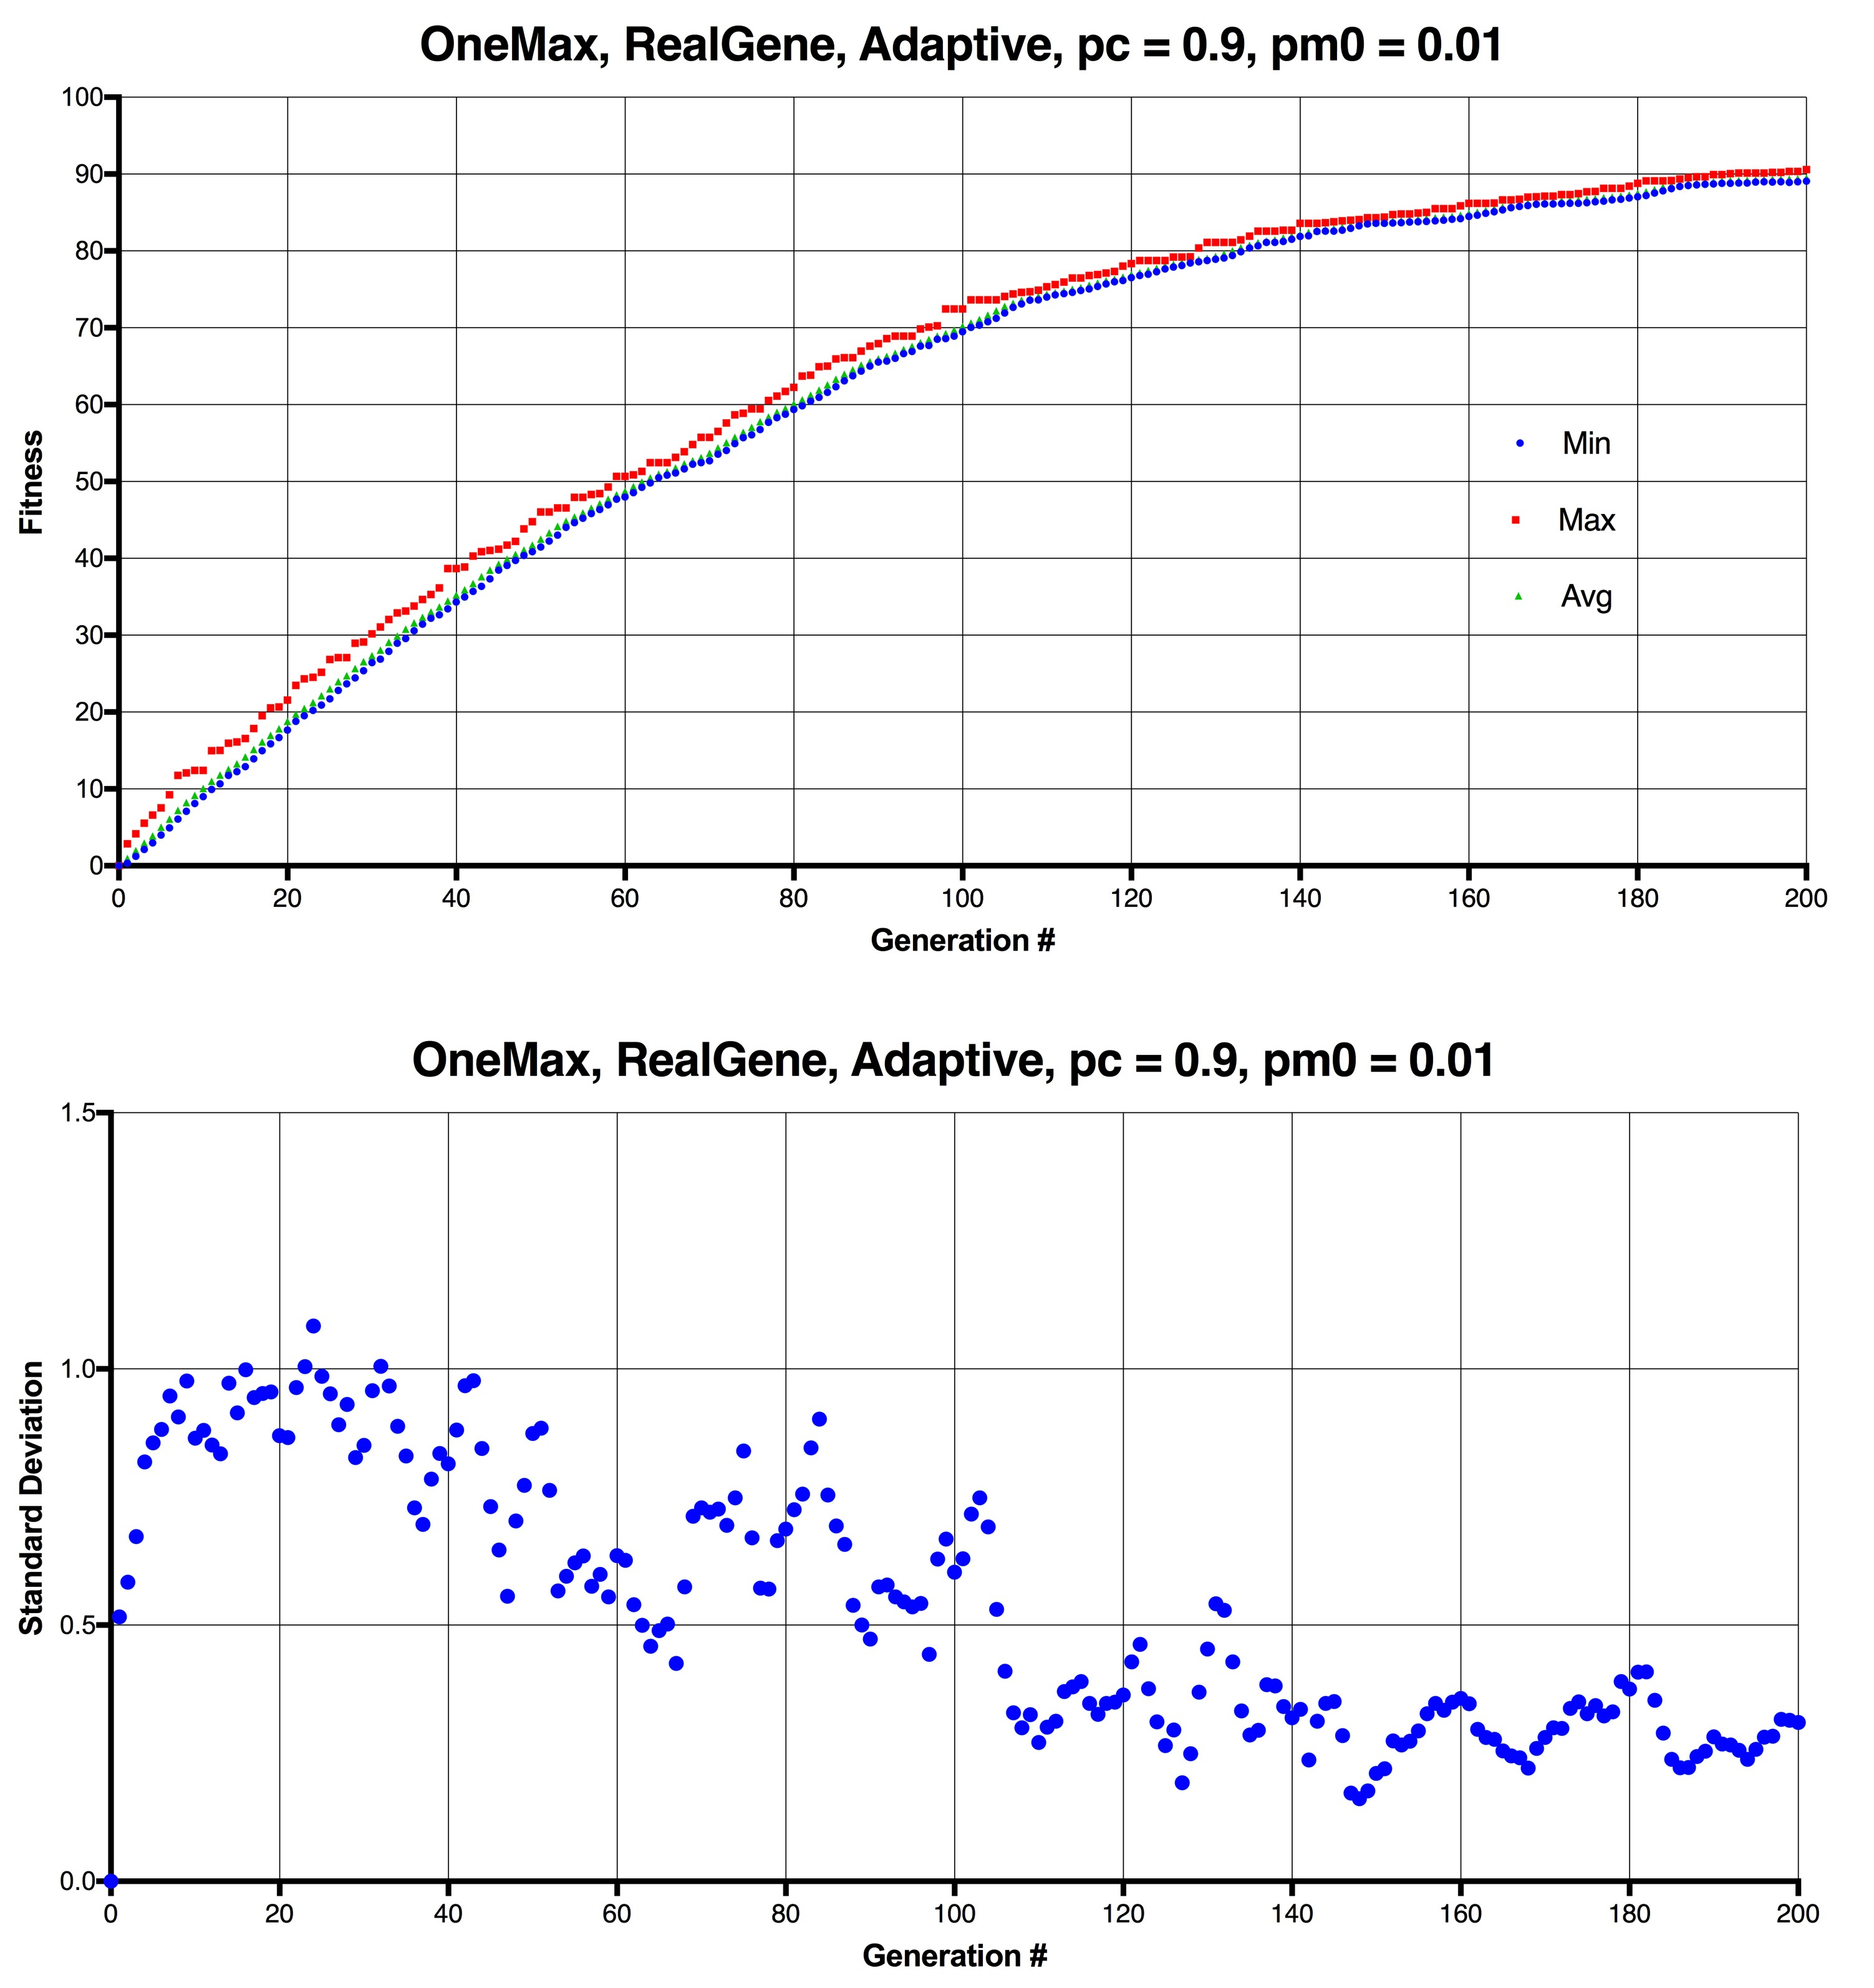
\includegraphics[width=1.0\textwidth]{onemax_real_adaptive.jpg}
    \caption{Evolução do fitness para o problema do OneMax Real Adaptativo mostrando mínimo, máximo, valor médio e desvio padrão ($p_c=0.9$, ${p_m}_0=0.01$).}
    \label{fig:onemax_real_adaptive}
\end{figure}

Observando a evolução de $p_m$ na figura \ref{fig:onemax_real_adaptive_pm}, vemos que, até que a população alcançasse o desvio traçado por ${p_m}_0$, foram necessárias mais de 140 gerações, justificando o crescimento inicial mais lento da população. No entanto, próximo de se atingir 200 gerações, $p_m$ cresceu e se aproximou cada vez mais de ${p_m}_0$, o que aumentou o fitness médio de modo mais rápido (aproximando-o do caso estático). Em termos de performance, o AGA mostrou aqui melhores resultados para o OneMax Real do que para o OneMax Booleano.

\begin{figure}[ht!]
    \centering 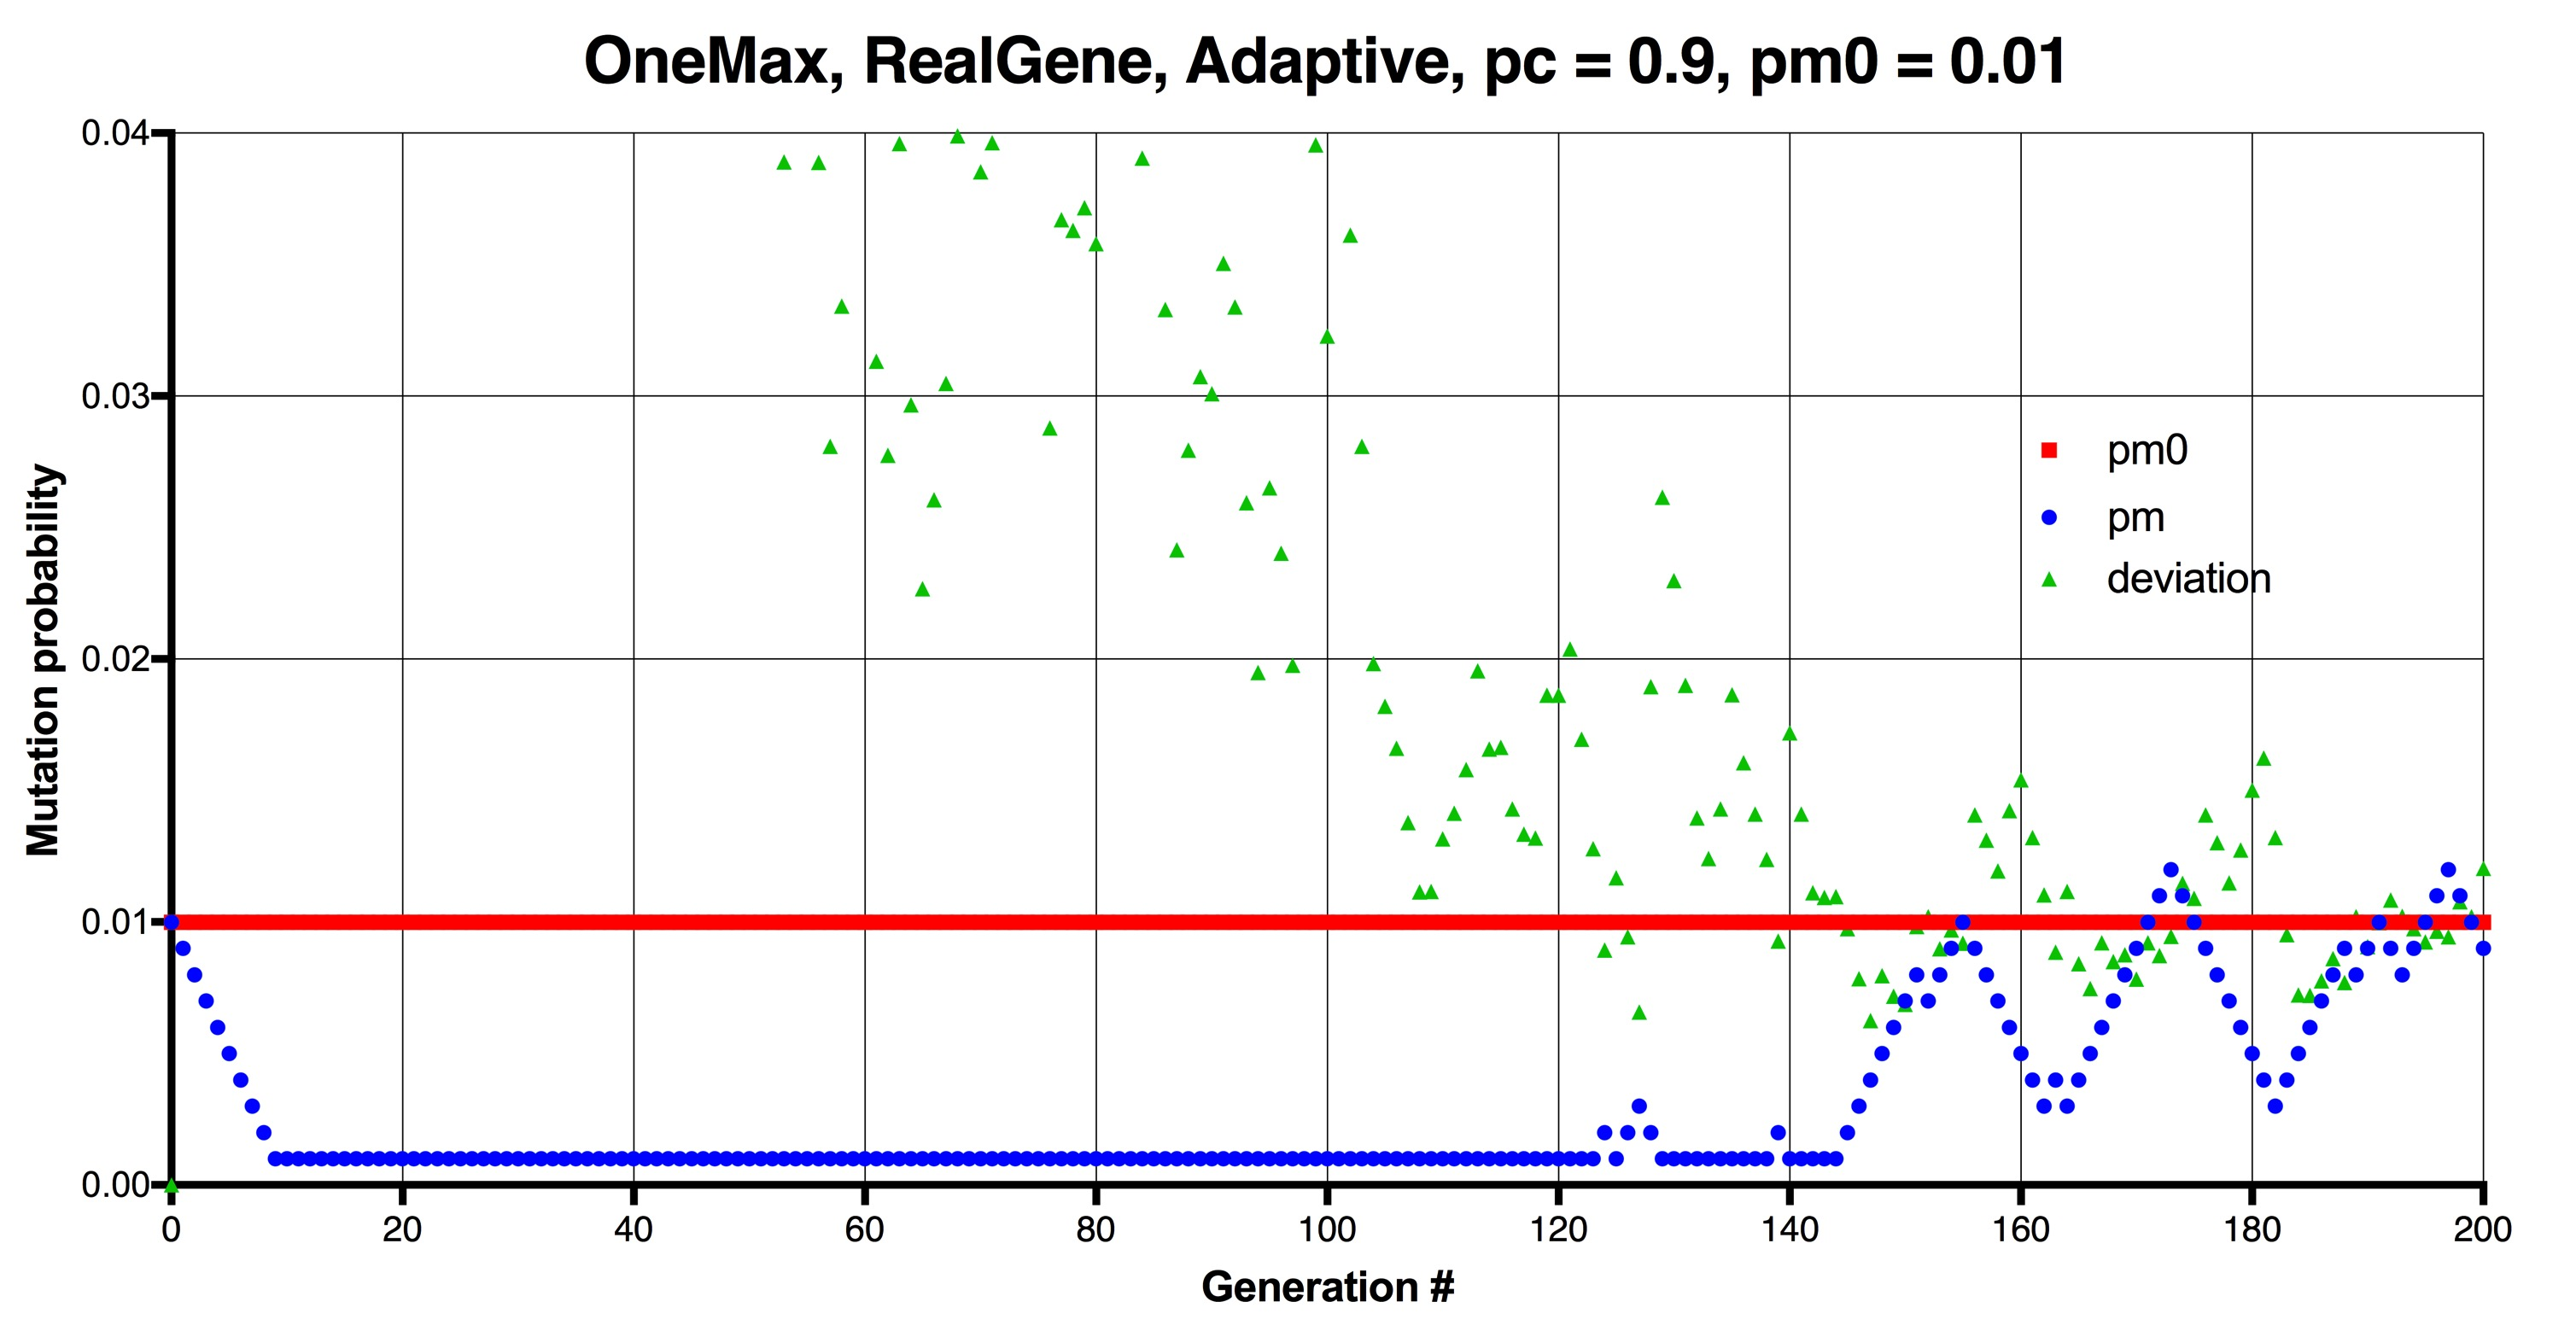
\includegraphics[width=1.0\textwidth]{onemax_real_adaptive_pm.jpg}
    \caption{Probabilidade de mutação ao longo das gerações para o problema do OneMax Real Adaptativo ($p_c=0.9$, ${p_m}_0=0.01$).}
    \label{fig:onemax_real_adaptive_pm}
\end{figure}

Os dados de interesse vindos destas simulações podem ser encontrados na tabela  \ref{tab:onemax_real}.

\begin{table}
\caption{Dados coletados do problema do OneMax Real ($p_m = 0.01$).}
\label{tab:onemax_real}

\center
\begin{tabular}{|c|cc|}
	\hline
	Algoritmo analisado (AG = caso estático) 	& AG		& AGA		\\
	\hline
	Fitness máximo após 100 gerações			& $85.115$	& $72.452$	\\
	Fitness médio após 100 gerações				& $84.048$	& $70.186$	\\
	Fitness máximo após 200 gerações 			& $93.083$	& $90.585$	\\
	Fitness médio após 200 gerações 			& $92.355$	& $89.507$	\\
	Valor final de $p_m$						& $0.01$ 	& $0.009$	\\
	Valor mínimo de $p_m$						& $0.01$	& $0.001$	\\
	Valor máximo de $p_m$						& $0.01$	& $0.012$	\\
	Valor médio de $p_m$						& $0.01$	& $0.00300$	\\
	Valor médio de $p_m$ (últimas 100 gerações)	& $0.01$	& $0.00458$	\\
	\hline
\end{tabular}
\end{table}

\section{Caixeiro Viajante Adaptado}

Para as simulações deste problema, utilizou-se o grafo do programa Open-Source DEAP com 17 cidades \cite{DEAP_JMLR2012, deap2016tsp}. Tal grafo é conexo, completo e bidirecionado, e sua distância mínima (começando na primeira cidade) é 2085. Ele está presente na listagem \ref{lst:cidades}.

\begin{lstlisting}[float, floatplacement=H, caption={Mapa de cidades para o problema do Caixeiro Viajante Adaptado.}, label=lst:cidades]
[0, 633, 257, 91, 412, 150, 80, 134, 259, 505, 353, 324, 70, 211, 268, 246, 121],
[633, 0, 390, 661, 227, 488, 572, 530, 555, 289, 282, 638, 567, 466, 420, 745, 518],
[257, 390, 0, 228, 169, 112, 196, 154, 372, 262, 110, 437, 191, 74, 53, 472, 142],
[91, 661, 228, 0, 383, 120, 77, 105, 175, 476, 324, 240, 27, 182, 239, 237, 84],
[412, 227, 169, 383, 0, 267, 351, 309, 338, 196, 61, 421, 346, 243, 199, 528, 297],
[150, 488, 112, 120, 267, 0, 63, 34, 264, 360, 208, 329, 83, 105, 123, 364, 35],
[80, 572, 196, 77, 351, 63, 0, 29, 232, 444, 292, 297, 47, 150, 207, 332, 29],
[134, 530, 154, 105, 309, 34, 29, 0, 249, 402, 250, 314, 68, 108, 165, 349, 36],
[259, 555, 372, 175, 338, 264, 232, 249, 0, 495, 352, 95, 189, 326, 383, 202, 236],
[505, 289, 262, 476, 196, 360, 444, 402, 495, 0, 154, 578, 439, 336, 240, 685, 390],
[353, 282, 110, 324, 61, 208, 292, 250, 352, 154, 0, 435, 287, 184, 140, 542, 238],
[324, 638, 437, 240, 421, 329, 297, 314, 95, 578, 435, 0, 254, 391, 448, 157, 301],
[70, 567, 191, 27, 346, 83, 47, 68, 189, 439, 287, 254, 0, 145, 202, 289, 55],
[211, 466, 74, 182, 243, 105, 150, 108, 326, 336, 184, 391, 145, 0, 57, 426, 96],
[268, 420, 53, 239, 199, 123, 207, 165, 383, 240, 140, 448, 202, 57, 0, 483, 153],
[246, 745, 472, 237, 528, 364, 332, 349, 202, 685, 542, 157, 289, 426, 483, 0, 336],
[121, 518, 142, 84, 297, 35, 29, 36, 236, 390, 238, 301, 55, 96, 153, 336, 0]
\end{lstlisting}

\subsection{Caso Estático ($p_m = 0.01$)}

Para o caso estático com $p_m = 0.01$, mostrado na figura \ref{fig:tsp001}, vemos que este valor de $p_m$ incentivou pouco o encontro de melhores soluções (pontos azuis), "travando" em um mesmo valor por 118 gerações. Em termos de desvio padrão, percebeu-se que $p_m = 0.01$ trouxe desvio zero bem mais rápido do que para um problema OneMax, uma vez que apenas 15 genes precisavam ser recombinados.

\begin{figure}[ht!]
    \centering 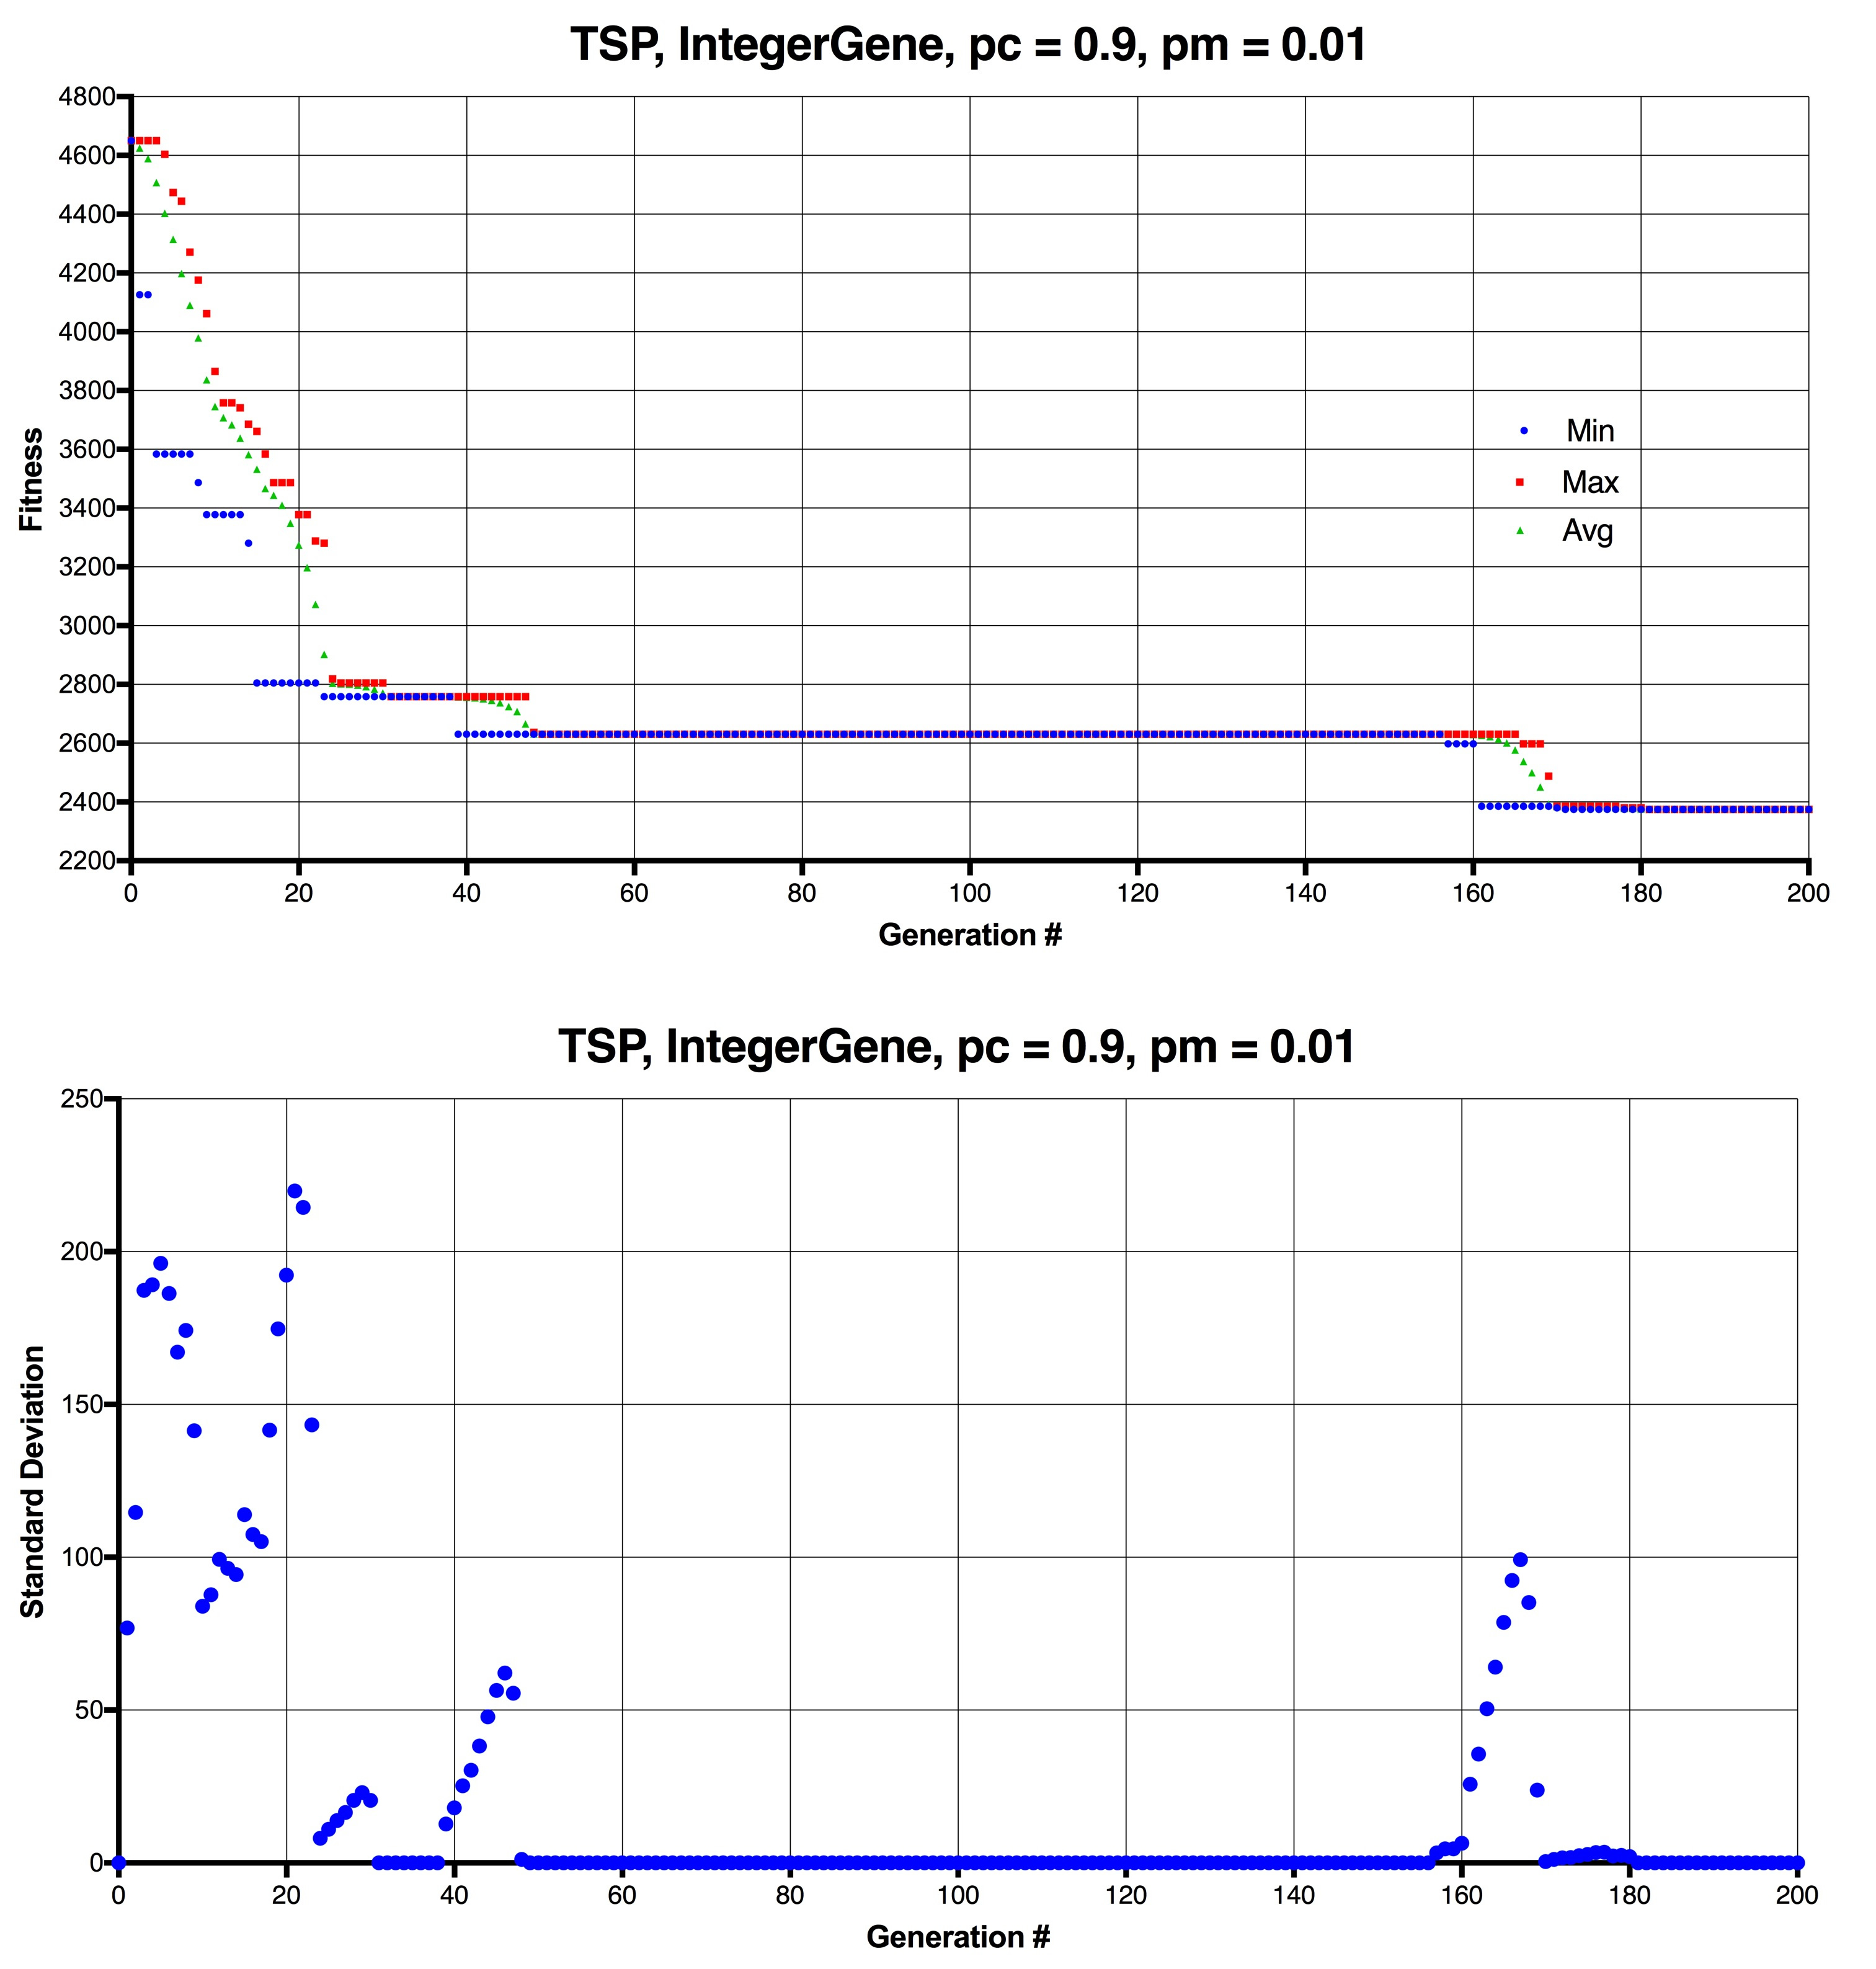
\includegraphics[width=1.0\textwidth]{tsp_001.jpg}
    \caption{Evolução do fitness para o problema do Caixeiro Viajante Adaptado, mostrando mínimo, máximo, valor médio e desvio padrão ($p_c=0.9$, $p_m=0.01$). O menor caminho encontrado tem distância total de 2375.}
    \label{fig:tsp001}
\end{figure}

Uma possível interpretação para o comportamento deste gráfico, considerando parâmetros estáticos, foi a de que o AG não conseguiria sair tão facilmente de um mínimo local para este valor de $p_m$. Uma possível solução seria a de aumentar $p_m$ e ver se ele seria capaz de trazer mais soluções. Com isso, analisou-se também o que aconteceria para este problema com $p_m = 0.2$ (20\% de mutação, muito mais intensa).

\subsection{Caso Estático ($p_m = 0.2$)}

Para o caso estático com $p_m = 0.2$, mostrado na figura \ref{fig:tsp02}, vemos uma solução melhor (2300 contra 2375 para $p_m = 0.01$). No entanto, o comportamento do melhor indivíduo não foi diferente daquele visto para $p_m = 0.01$, sendo que agora o AG ficou travado por 127 gerações. 

\begin{figure}[ht!]
    \centering 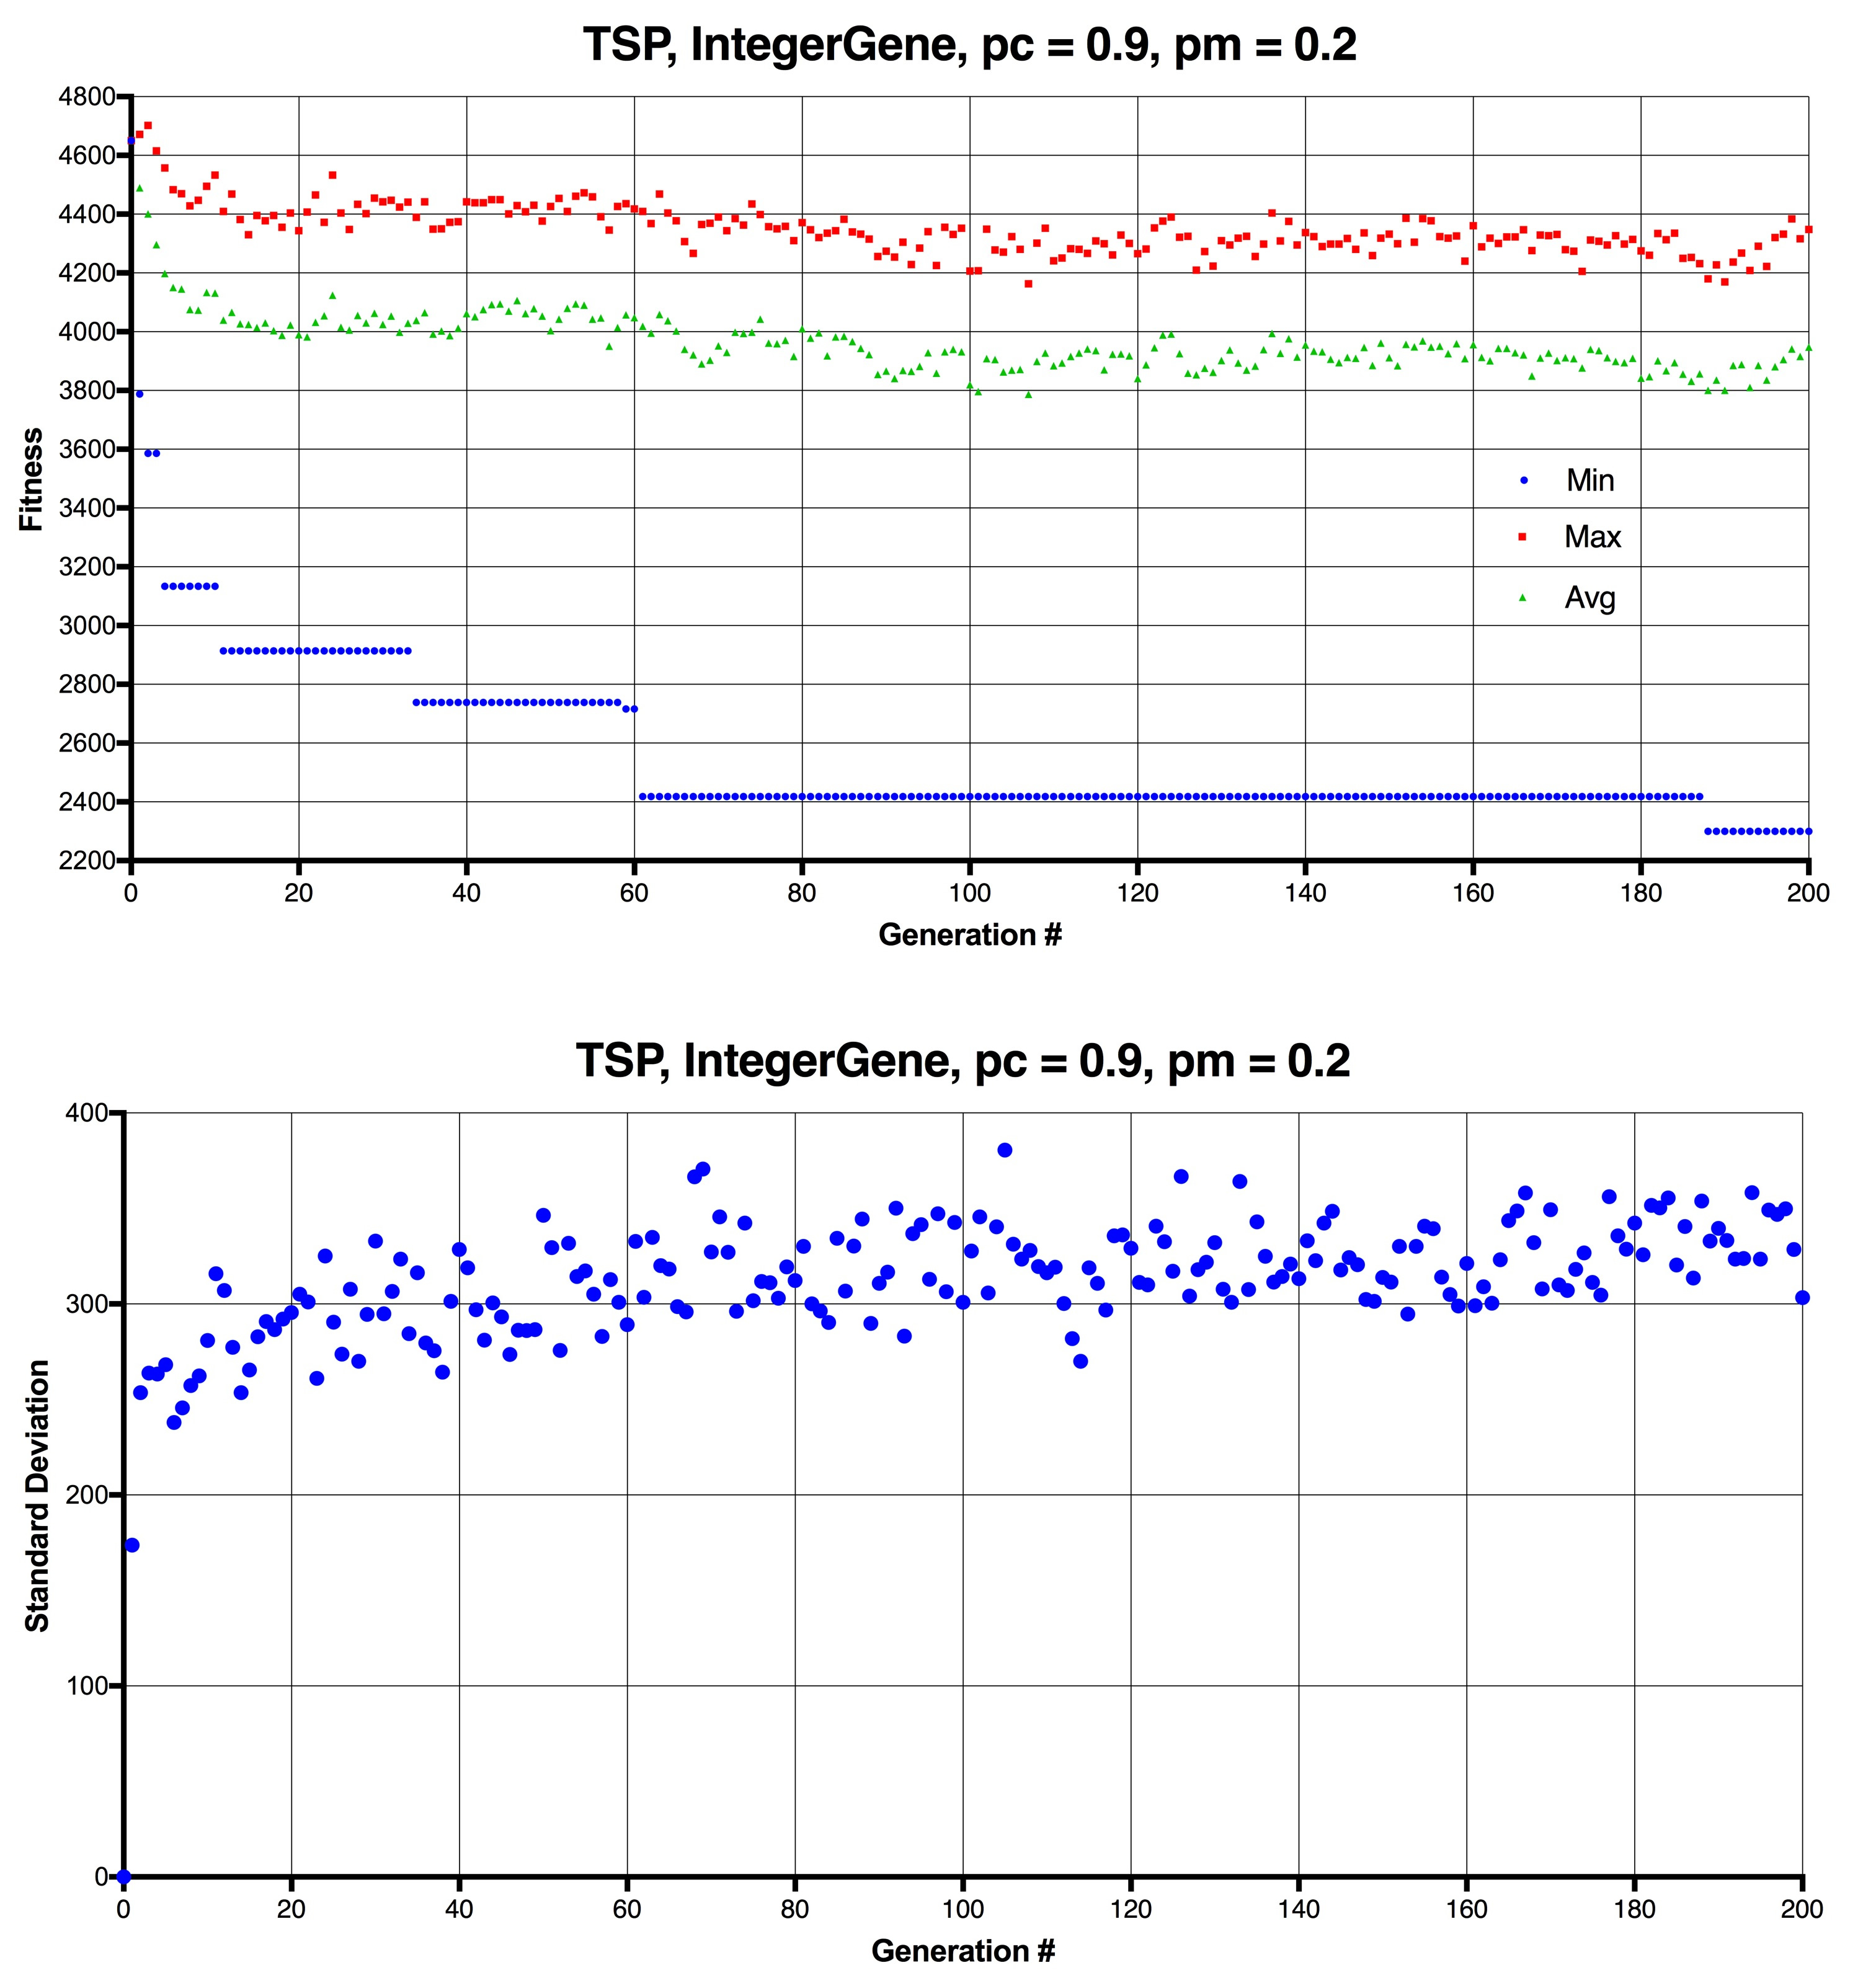
\includegraphics[width=1.0\textwidth]{tsp_02.jpg}
    \caption{Evolução do fitness para o problema do Caixeiro Viajante Adaptado, mostrando mínimo, máximo, valor médio e desvio padrão ($p_c=0.9$, $p_m=0.2$). O menor caminho encontrado tem distância total de 2300.}
    \label{fig:tsp02}
\end{figure}

A curva de desvio padrão nos sugere que a população foi capaz de encontrar bem mais soluções. No entanto, com uma mutação mais intensa, tais soluções são ainda mais imprevisíveis aos olhos do problema, o que nos fez ver que aumentar $p_m$ não fez diferença para o caso estático.

\subsection{Caso Adaptativo ($p_m = 0.01$)}

O caso adaptativo para $p_m = 0.01$ mostrou uma evolução bem diferente do caso estático. Como visto na figura \ref{fig:tsp_001_adaptative}, a população também conseguiu se homogeneizar de tempos em tempos, mas o melhor indivíduo encontrou novas soluções muito mais rapidamente. A melhor solução foi mantida por não mais de 69 gerações, com um fitness mínimo final melhor do que aqueles do caso estático (2287 contra 2375 para $p_m = 0.01$ e 2300 para $p_m = 0.2$).

\begin{figure}[ht!]
    \centering 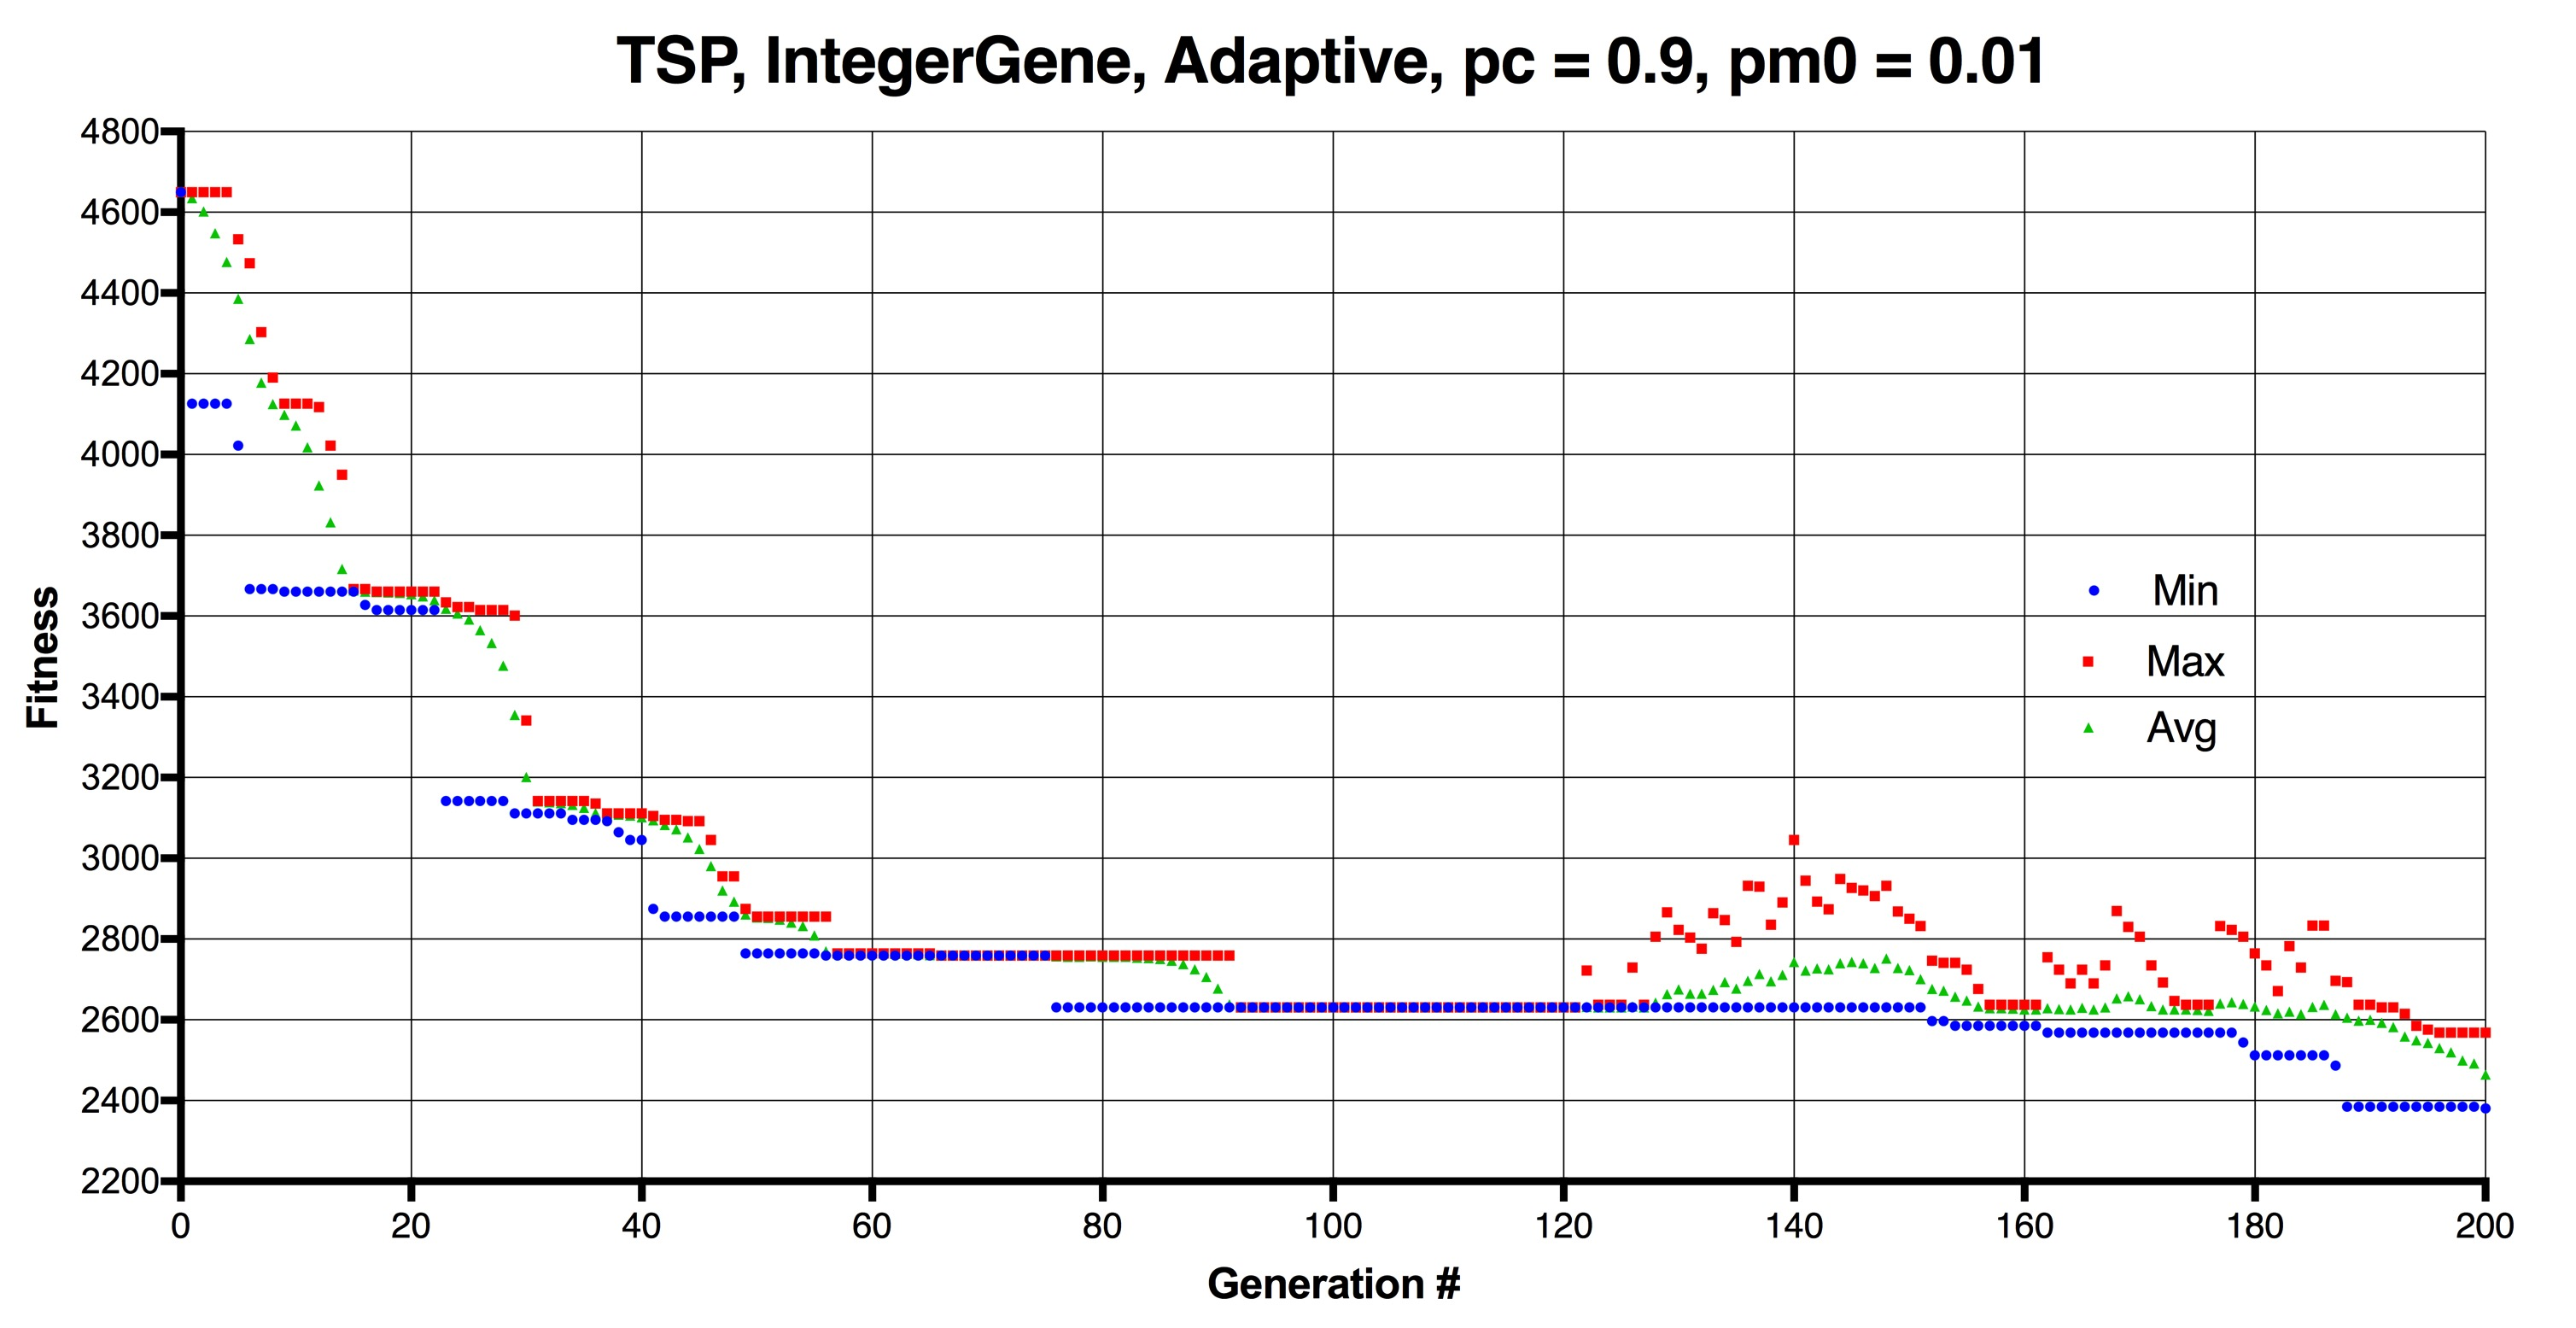
\includegraphics[width=1.0\textwidth]{tsp_001_adaptive.jpg}
    \caption{Evolução do fitness para o caso adaptativo do problema do Caixeiro Viajante Adaptado, mostrando mínimo, máximo, valor médio e desvio padrão ($p_c=0.9$, ${p_m}_0=0.01$). O menor caminho encontrado tem distância total de 2287.}
    \label{fig:tsp_001_adaptative}
\end{figure}

A evolução de $p_m$ mostrada na figura \ref{fig:tsp_001_adaptive_pm} foi bem diferente daquela observada para os problemas OneMax. Como era muito fácil para a população se homogeneizar, $p_m$ chegou a valores maiores que 0.05 e oscilou muito. No entanto, este AGA foi feito para impedir que a população travasse em uma mesma solução, e este efeito ficou evidente nesta simulação, com os desvios (em verde) mudando abruptamente de valor conforme $p_m$ aumenta. Tal comportamento do AGA se mostrou eficaz e decisivo no encontro de melhores soluções para o problema do Caixeiro Viajante Adaptado.

\begin{figure}[ht!]
    \centering 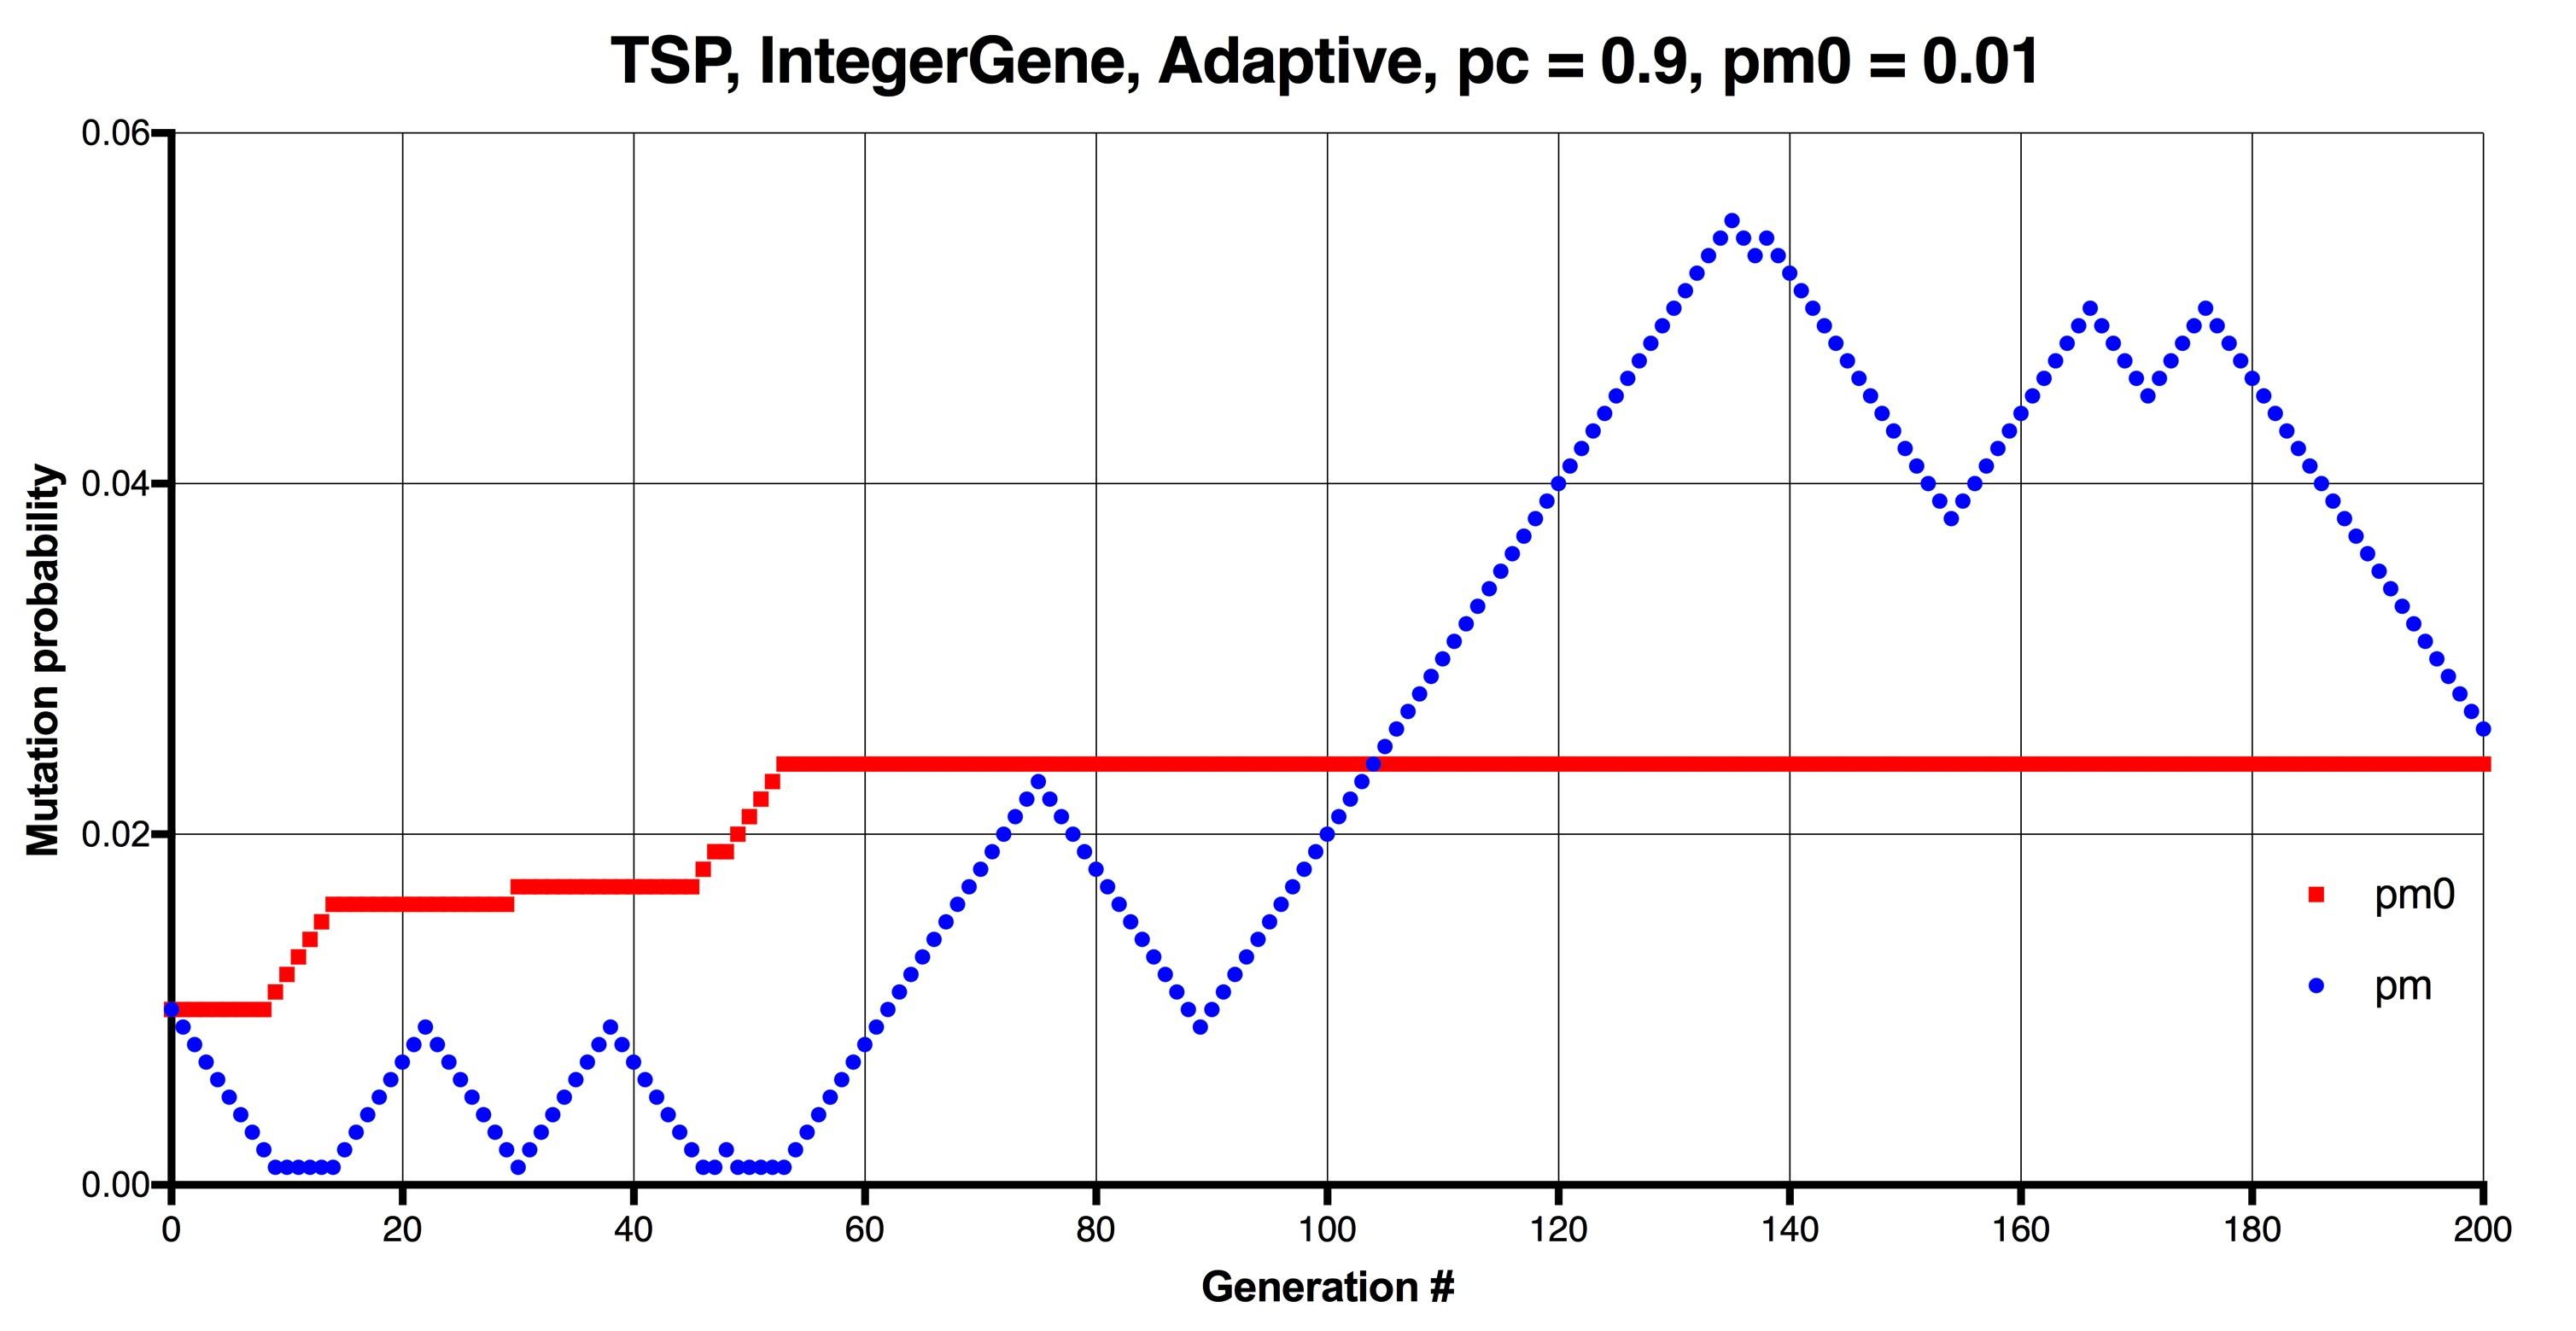
\includegraphics[width=1.0\textwidth]{tsp_001_adaptive_pm.jpg}
    \caption{Probabilidade de mutação ao longo das gerações para o caso adaptativo do problema do Caixeiro Viajante Adaptado ($p_c=0.9$, ${p_m}_0=0.01$).}
    \label{fig:tsp_001_adaptive_pm}
\end{figure}

Como foram feitas duas simulações para o caso estático, optou-se por analisar também o caso adaptativo para $p_m = 0.2$.

\subsection{Caso Adaptativo ($p_m = 0.2$)}

O gráfico da figura \ref{fig:tsp_02_adaptative} encontrou o menor percurso dentre as simulações feitas aqui (2138). As melhores soluções foram mantidas por, no máximo, 33 gerações. Não só isso, todas as curvas (mínimo, máximo e média) evoluíram de formas semelhante, mesmo com uma mutação inicial intensa. A curva do desvio padrão, apesar de manter valores altos, mostrou também uma tendência de queda nas últimas gerações.

\begin{figure}[ht!]
    \centering 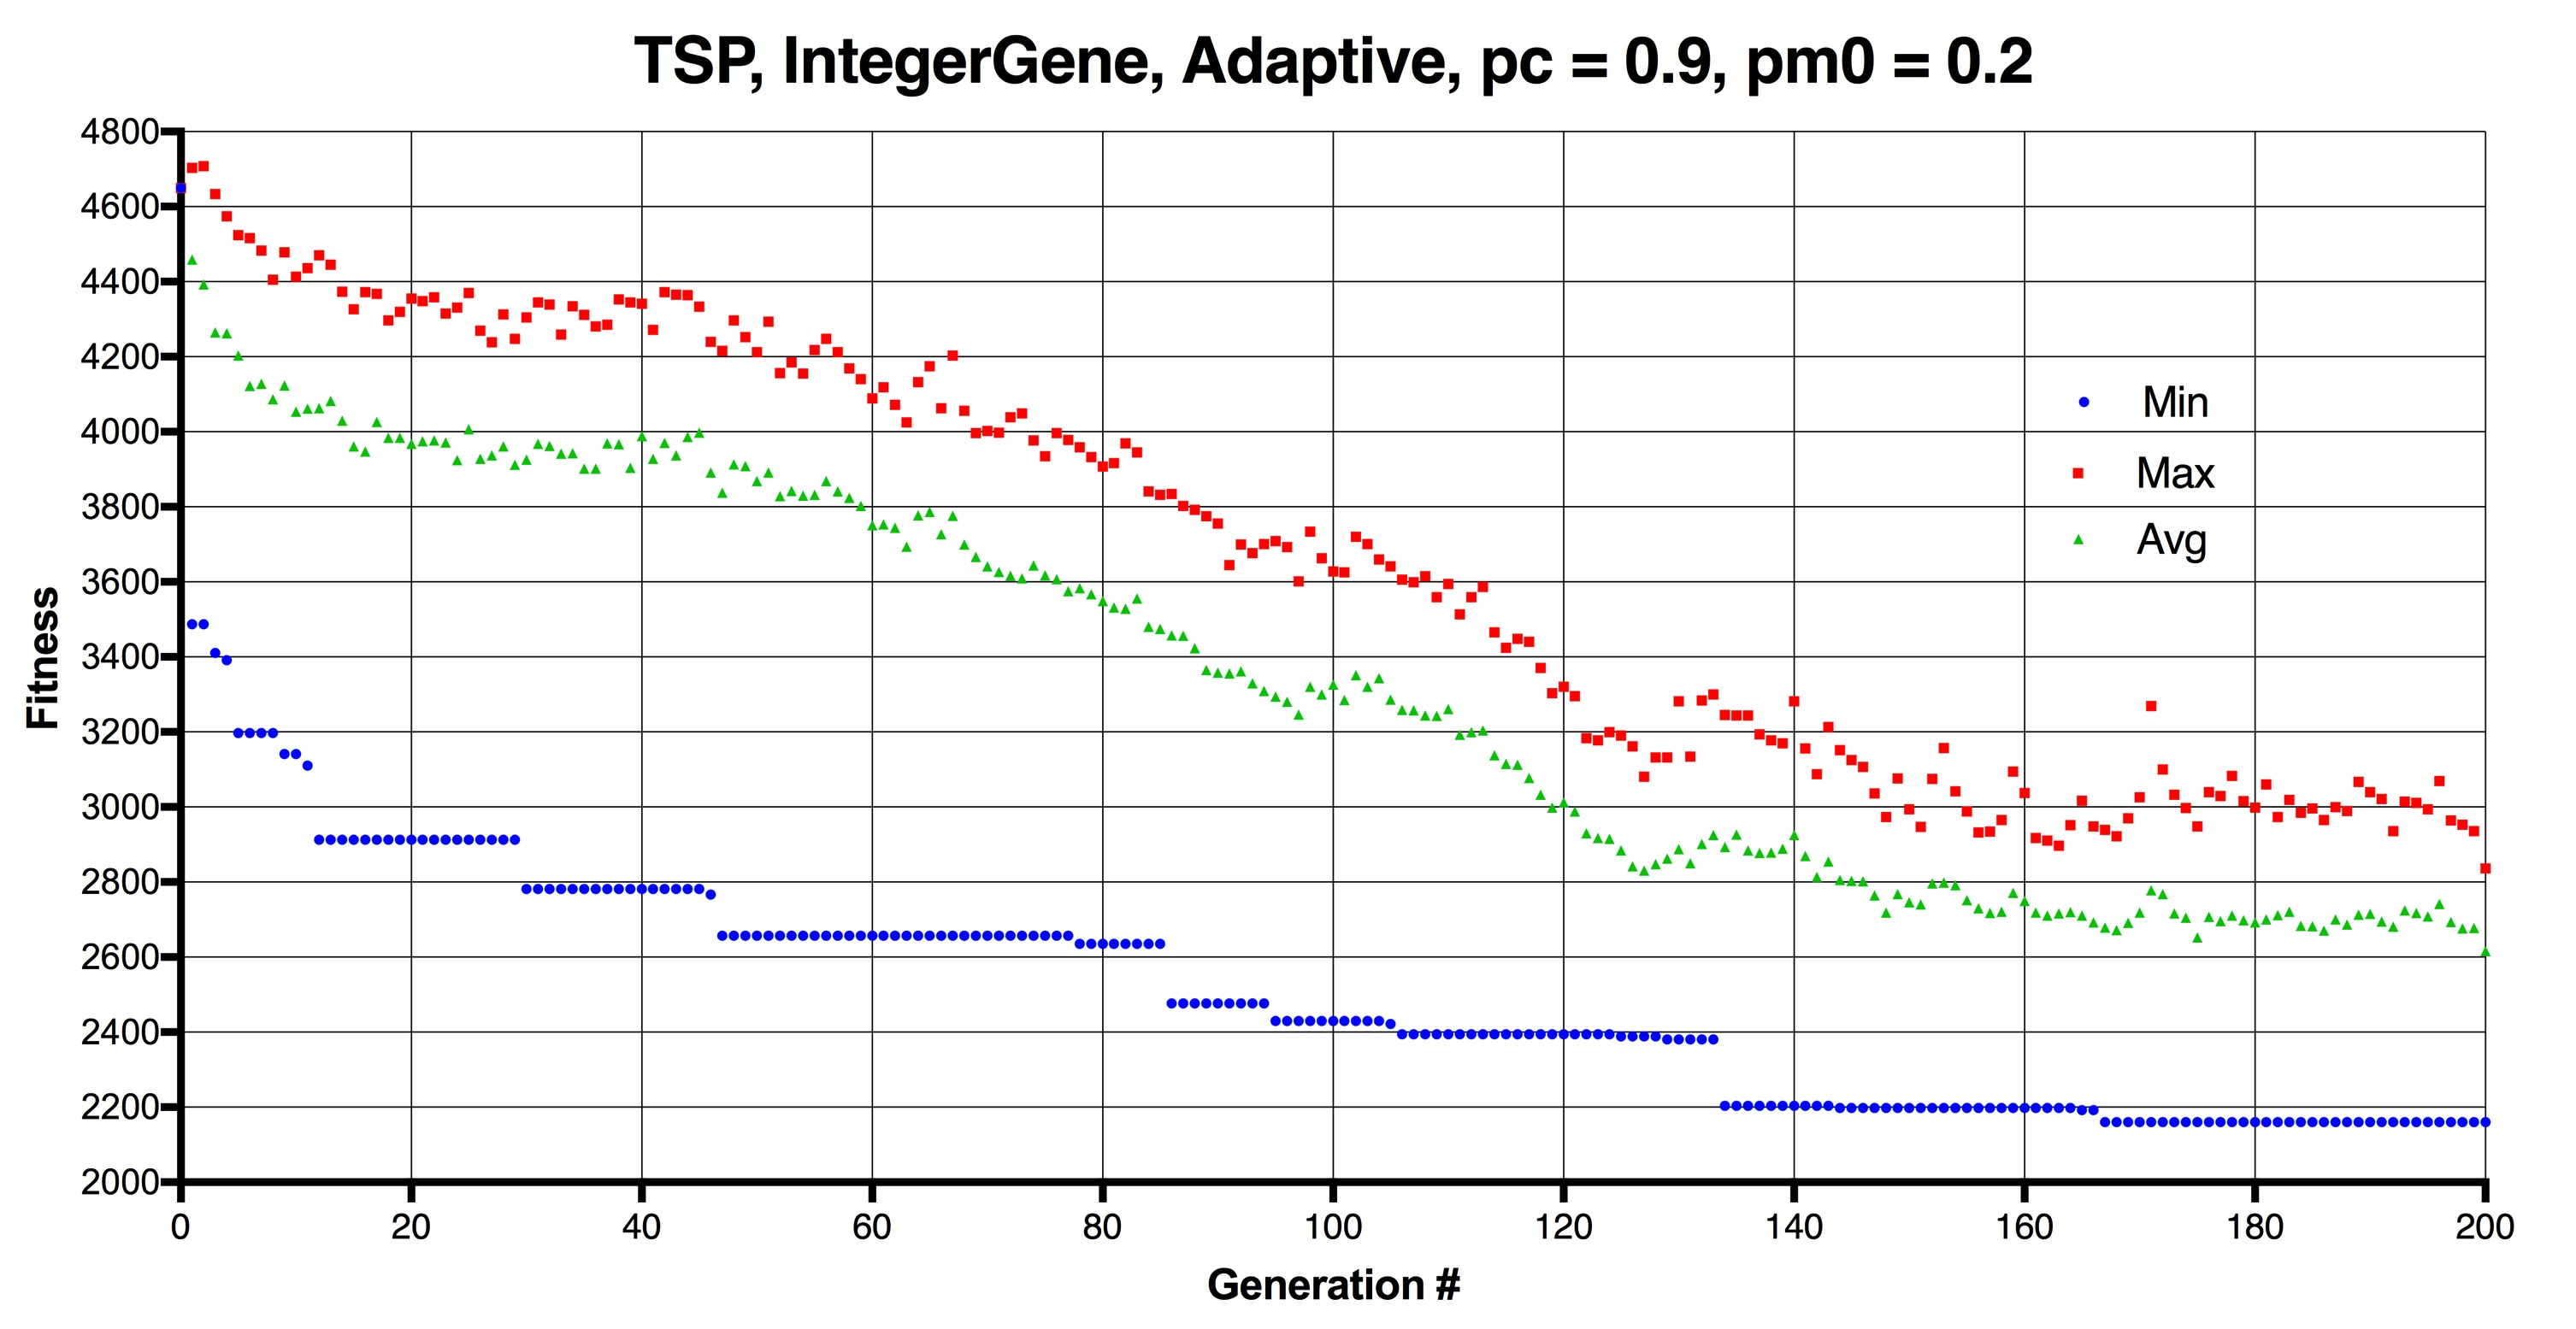
\includegraphics[width=1.0\textwidth]{tsp_02_adaptive.jpg}
    \caption{Evolução do fitness para o caso adaptativo do problema do Caixeiro Viajante Adaptado, mostrando mínimo, máximo, valor médio e desvio padrão ($p_c=0.9$, ${p_m}_0=0.2$). O menor caminho encontrado tem distância total de 2138.}
    \label{fig:tsp_02_adaptative}
\end{figure}

A curva de interesse aqui foi certamente a da figura \ref{fig:tsp_02_adaptive_pm}. O valor de $p_m$ diminuiu diretamente para uma faixa estável em torno de seu valor final (0.0866). Esta é a curva que melhor demonstra o potencial do AGA desenvolvido aqui: mesmo começando num valor desfavorável para convergência, $p_m$ mudou de patamar e foi estabilizado, trazendo a melhor resposta para o desvio e a melhor evolução para este problema em 200 gerações.

\begin{figure}[ht!]
    \centering 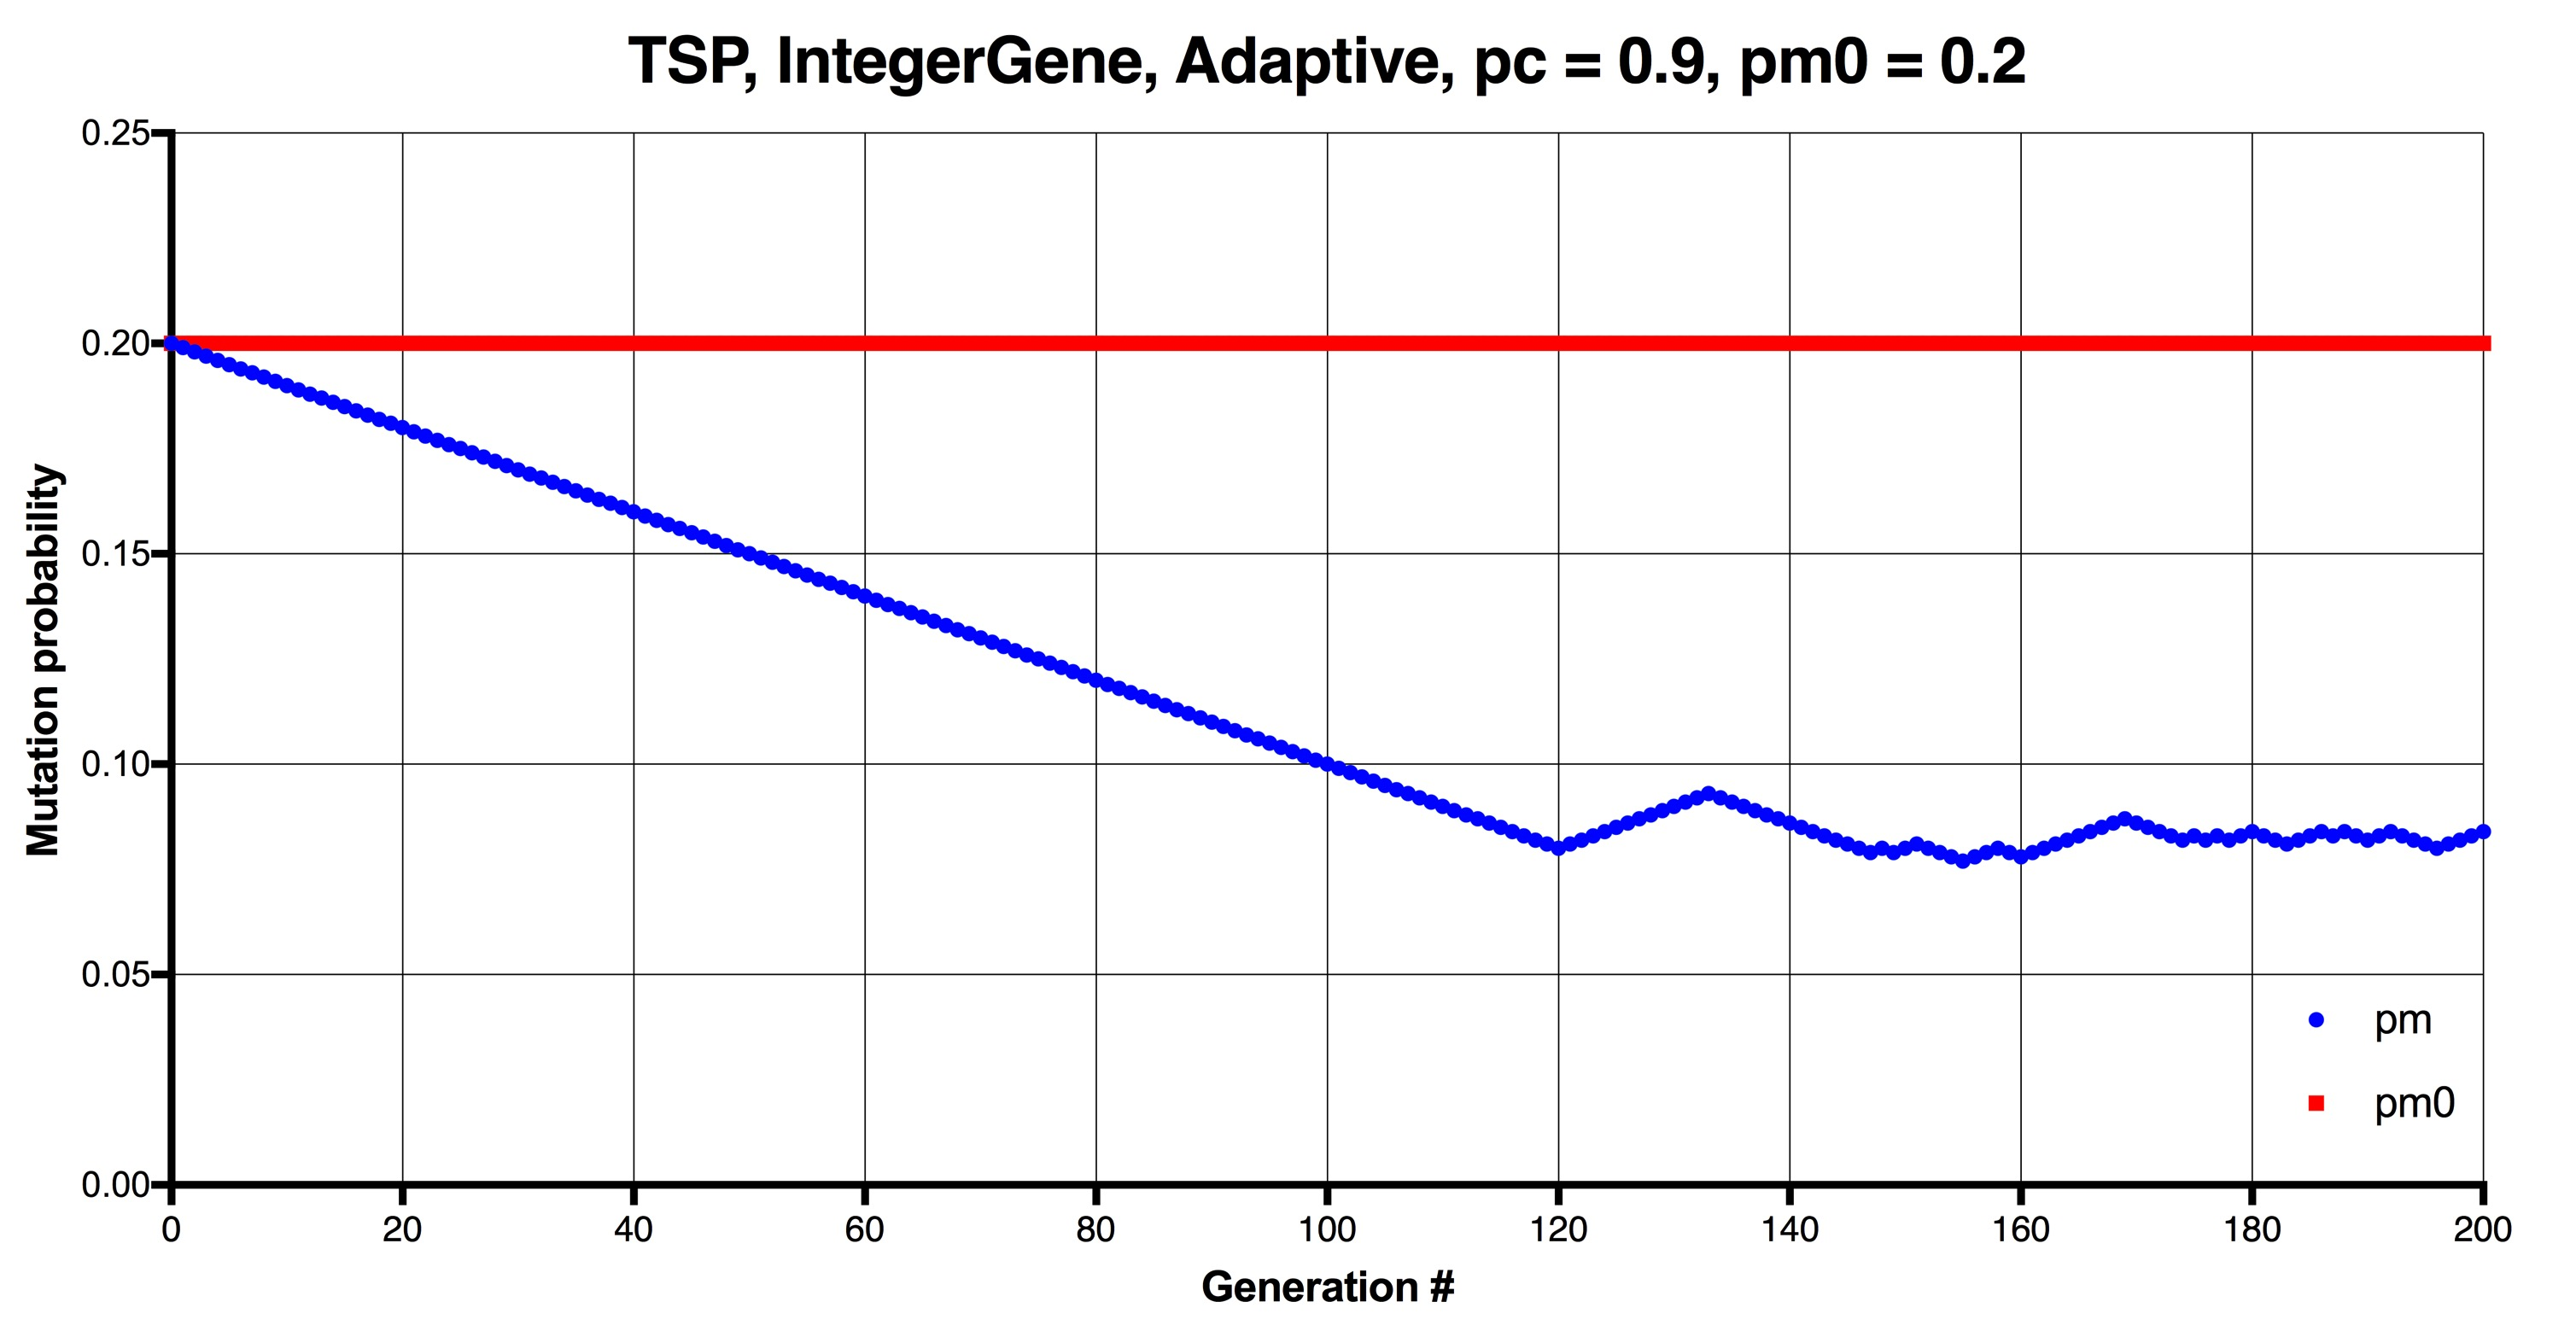
\includegraphics[width=1.0\textwidth]{tsp_02_adaptive_pm.jpg}
    \caption{Probabilidade de mutação ao longo das gerações para o caso adaptativo do problema do Caixeiro Viajante Adaptado ($p_c=0.9$, ${p_m}_0=0.2$).}
    \label{fig:tsp_02_adaptive_pm}
\end{figure}

Os dados de interesse destas quatro simulações estão presentes na tabela \ref{tab:tsp}.

\begin{table}
\caption{Dados coletados do problema do Caixeiro Viajante Adaptado.}
\label{tab:tsp}

\centering
\begin{tabular}[!hbt]{|c|cc|cc|}
	\hline
	Valor inicial de $p_m$						& \multicolumn{2}{c|}{0.01}		& \multicolumn{2}{c|}{0.2}		\\
	\hline
	Algoritmo analisado (AG = caso estático)	& AG			& AGA			& AG			& AGA			\\
	\hline
	Fitness mínimo após 100 gerações			& $2631$		& $2631$		& $2418$		& $2379$		\\
	Fitness médio após 100 gerações				& $2631$		& $2701.2$		& $3819.5$		& $3267.64$		\\
	Fitness mínimo após 200 gerações 			& $2375$		& $2287$		& $2300$		& $2138$		\\
	Fitness médio após 200 gerações 			& $2375$		& $2349.11$		& $3948.11$		& $2621.33$		\\
	\# máximo de gerações "travado" (fitness)	& $118 (2631)$	& $69 (2631)$	& $127 (2418)$	& $33 (2661)$	\\
	Valor final de $p_m$						& $0.01$		& $0.043$		& $0.2$			& $0.078$		\\
	Valor mínimo de $p_m$						& $0.01$		& $0.001$		& $0.2$			& $0.072$		\\
	Valor máximo de $p_m$						& $0.01$		& $0.055$		& $0.2$			& $0.204$		\\
	Valor médio de $p_m$						& $0.01$		& $0.0261$		& $0.2$			& $0.122$		\\
	Valor médio de $p_m$ (últimas 100 gerações)	& $0.01$		& $0.0327$		& $0.2$			& $0.0866$		\\
	\hline
\end{tabular}
\end{table}

\section{Discussões}

Os três problemas foram simulados tanto pelo AG estático quanto pelo AGA. Para os problemas OneMax, foi possível observar uma evolução melhor para o caso estático do que para o caso adaptativo. Para o problema do Caixeiro Viajante Adaptado, no entanto, o AGA mostrou resultados muito melhores. Seria possível validar o AGA a partir destes experimentos?

Pensemos nas operações de variação de um AG. Se associarmos probabilidade de crossover $p_c$ (alta) ao fator de homogeneização do fitness da população, então a probabilidade de mutação $p_m$, combinada com elitismo, pode atuar de duas formas:

\begin{itemize}
	\item Tornando a população heterogênea;
	\item \textbf{Melhorando o fitness do melhor indivíduo}.
\end{itemize}

O efeito que será mais predominante dependerá do valor de $p_m$ e do problema. Como visto no OneMax, um valor de 0.01 ou de 0.001 foi suficiente para priorizar o segundo efeito sobre o primeiro, evoluindo gradualmente o melhor indivíduo.

No entanto, o problema do Caixeiro Viajante Adaptado não conseguiu se beneficiar destes efeitos nem para $p_m=0.01$, nem para $p_m=0.2$. Não que o AG estático não possua um valor ideal para convergência deste problema em específico - isto apenas mostra que um parâmetro que funcione para um determinado problema não irá funcionar da mesma forma para outro problema.

Se tentássemos estressar o problema do Caixeiro Viajante para o caso estático, poderíamos eventualmente encontrar um valor ideal para $p_m$. No entanto, tal problema (mesmo adaptado) ainda é NP-Hard, e um valor estático de $p_m$ não se mostrou suficiente para encontrar melhores soluções. O que resolveria este problema, quando um valor muito baixo e um valor muito alto de ${p_m}_0$ não são suficientes?

Em busca de uma melhor performance, entra em cena um algoritmo adaptativo. Algo a se acrescentar ao AG que permitisse adaptar o valor de $p_m$ ao longo das gerações. Mesmo que o uso do AGA não trouxesse melhores soluções mais rapidamente, ele se mostrou melhor para "destravar" o AG de mínimos locais. No entanto, o uso do AGA não trouxe o mesmo benefício para os problemas OneMax. Repensar o AGA é uma ideia válida, mas usar o AGA será sempre uma ideia melhor?

Para isso, é necessário considerar os teoremas "No Free Lunch" (em português, esta expressão deu origem a "Não existe almoço grátis") \cite{wolpert1997no}. De maneira simples, estes teoremas dizem que, para um algoritmo de busca e otimização (como é o caso do AG e do AGA), uma performance elevada para um grupo de problemas (como os problemas OneMax) tem como preço uma queda de performance para os demais grupos de problemas (como o problema do Caixeiro Viajante Adaptado). O AGA tentaria ser a adaptação do AG para se adequar a outros problemas, e mesmo assim, ele veio com uma perda de performance para os problemas OneMax.

Não é possível utilizar o mesmo algoritmo para todos os problemas. Mesmo que não utilizássemos um AGA, ainda haveria formas melhores de se otimizar o AG para um grupo de problemas, incluindo o Caixeiro Viajante. Isso, no entanto, não tira os méritos do AGA.

Pelos experimentos feitos neste trabalho, ele foi capaz de encontrar soluções melhores para um problema mais complexo que os OneMax. Melhor performance é sempre interessante, mas ser capaz de encontrar soluções cada vez melhores é, ao olhos deste trabalho, muito melhor. Restaria então verificar se outros problemas conseguiriam se beneficiar do AGA da mesma forma, ou mesmo se o AGA não poderia ser melhorado. Até lá, temos bons resultados e análises interessantes vindas deste AGA.
